\section{Methods}
\label{sec:methods}

In this section, we present our \mm~ algorithm. We first discuss the choice of the stop condition for the recursive function and how matrices are being divided to smaller blocks. Then, We explain how the communication is being done in an overlapped distributed fashion to help the recursive function scale better.

%We then explain further modifications to the triple matrix multiplication (\ref{eq:rap}) that are part of the AMG setup process.

\subsection{Matrix-Matrix Multiplication}
\label{sec:matmult}

%\subsubsection{Computation}
%\label{sec:comp}
We design a divide and conquer approach to perform \textsc{GEMM} in a node-local fashion. The key idea is to perform simple tasks while recursing, having efficient memory access, and to perform the multiplication for small chunks where the resulting matrix can fit into an appropriate cache. For clarity of presentation, we assume that the data is available locally and discuss it as a serial implementation. Shared memory parallelism is added in a straightforward manner. The distributed part is explained in the next section. The matrices are stored in the \textit{CSC} sparse format.
%We have implemented \mm~ in a recursive fashion.
%We split the matrices recursively in two ways: split by half based on the matrix size and based on number of nonzeros. First we explain the algorithms performing splitting based on the matrix sizes.

To perform the multiplication
\begin{equation}
    C = A \times B
\end{equation}
we keep splitting the matrices horizontally and vertically (Figure~\ref{fig:split2}) based on row size and column size of $A$, until we can fit the result of the multiplication in a dense buffer.

\begin{figure}[tbh]
 \centering
 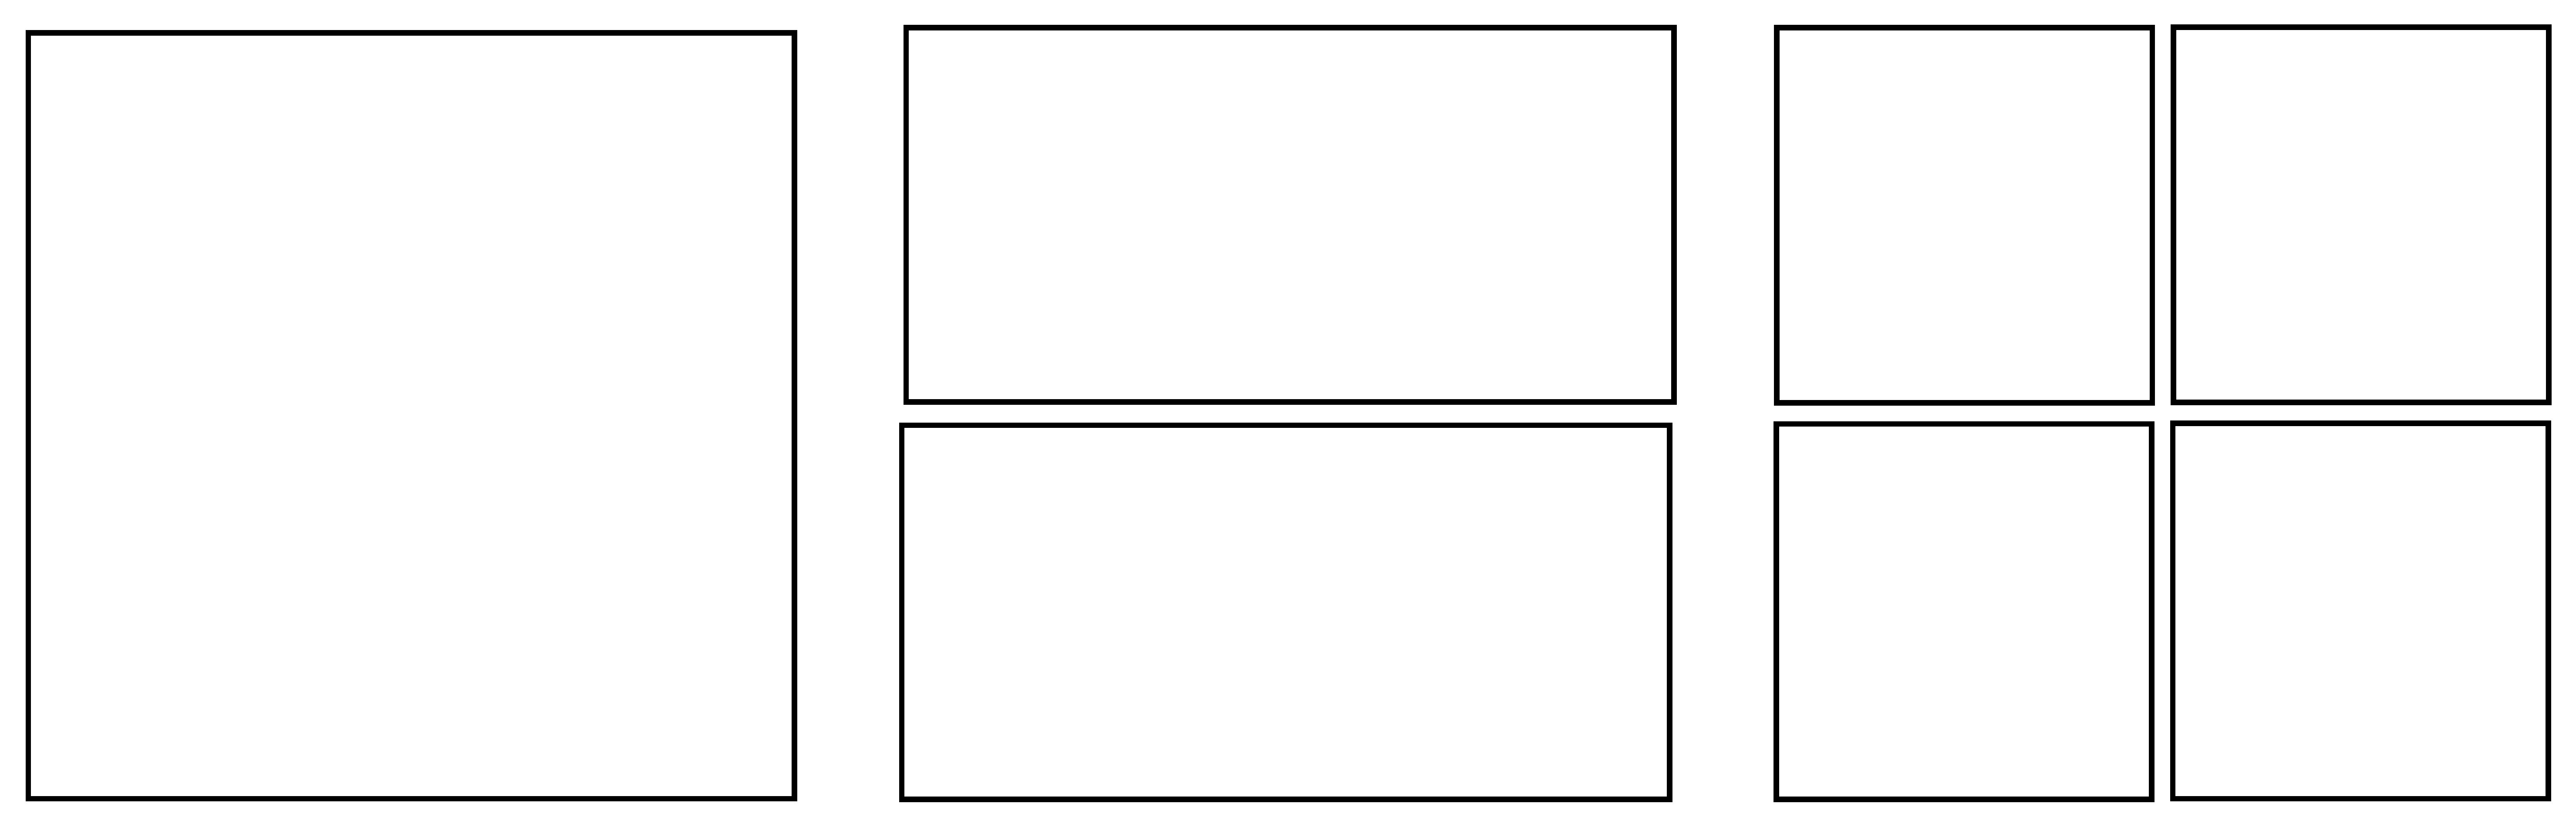
\includegraphics[width=8.5cm,height=2.7cm]{./figures/split2.pdf}
 \caption{A basic scheme that shows splitting the matrix first horizontally, then vertically.}
 \label{fig:split2}

\end{figure}

The recursive function, \recmm, includes three cases:
\begin{enumerate}
 \item Case 1: Stop the recursion and perform the multiplication.
 \item Case 2: $A$ is horizontal. Split the blocks.
 \item Case 3: $A$ is vertical. Split the blocks.
\end{enumerate}

\subsubsection{Case 1}
\label{sec:case1}
First we discuss when we decide to stop the recursive function.  
Our goal is to fit the multiplication result of blocks of $A$ and $B$ in a dense buffer. We show the blocks of $A$ and $B$ as $A_{ij}$ and $B_{lk}$. We use two indices here because the matrices get divided both horizontally and vertically. The size of the dense buffer to store $A_{ij} \times B_{lk}$ is
\begin{equation}
    row\ size\ of\ A_{ij} \times column\ size\ of\ B_{lk}\label{eq:thres}
\end{equation}

Therefore, Equation~ \eqref{eq:thres} can be used as the naive choice to decide when to stop the recursion, but Figure~\ref{fig:thres} shows why that is not a good choice. If we use Equation~ \eqref{eq:thres} for this example, the splitting process for the top two blocks of the matrix stops at the same step because they have the same size, but to have a more efficient method the top left block should be divided to more blocks than the top right block.

\begin{figure}[tbh]
 \centering
 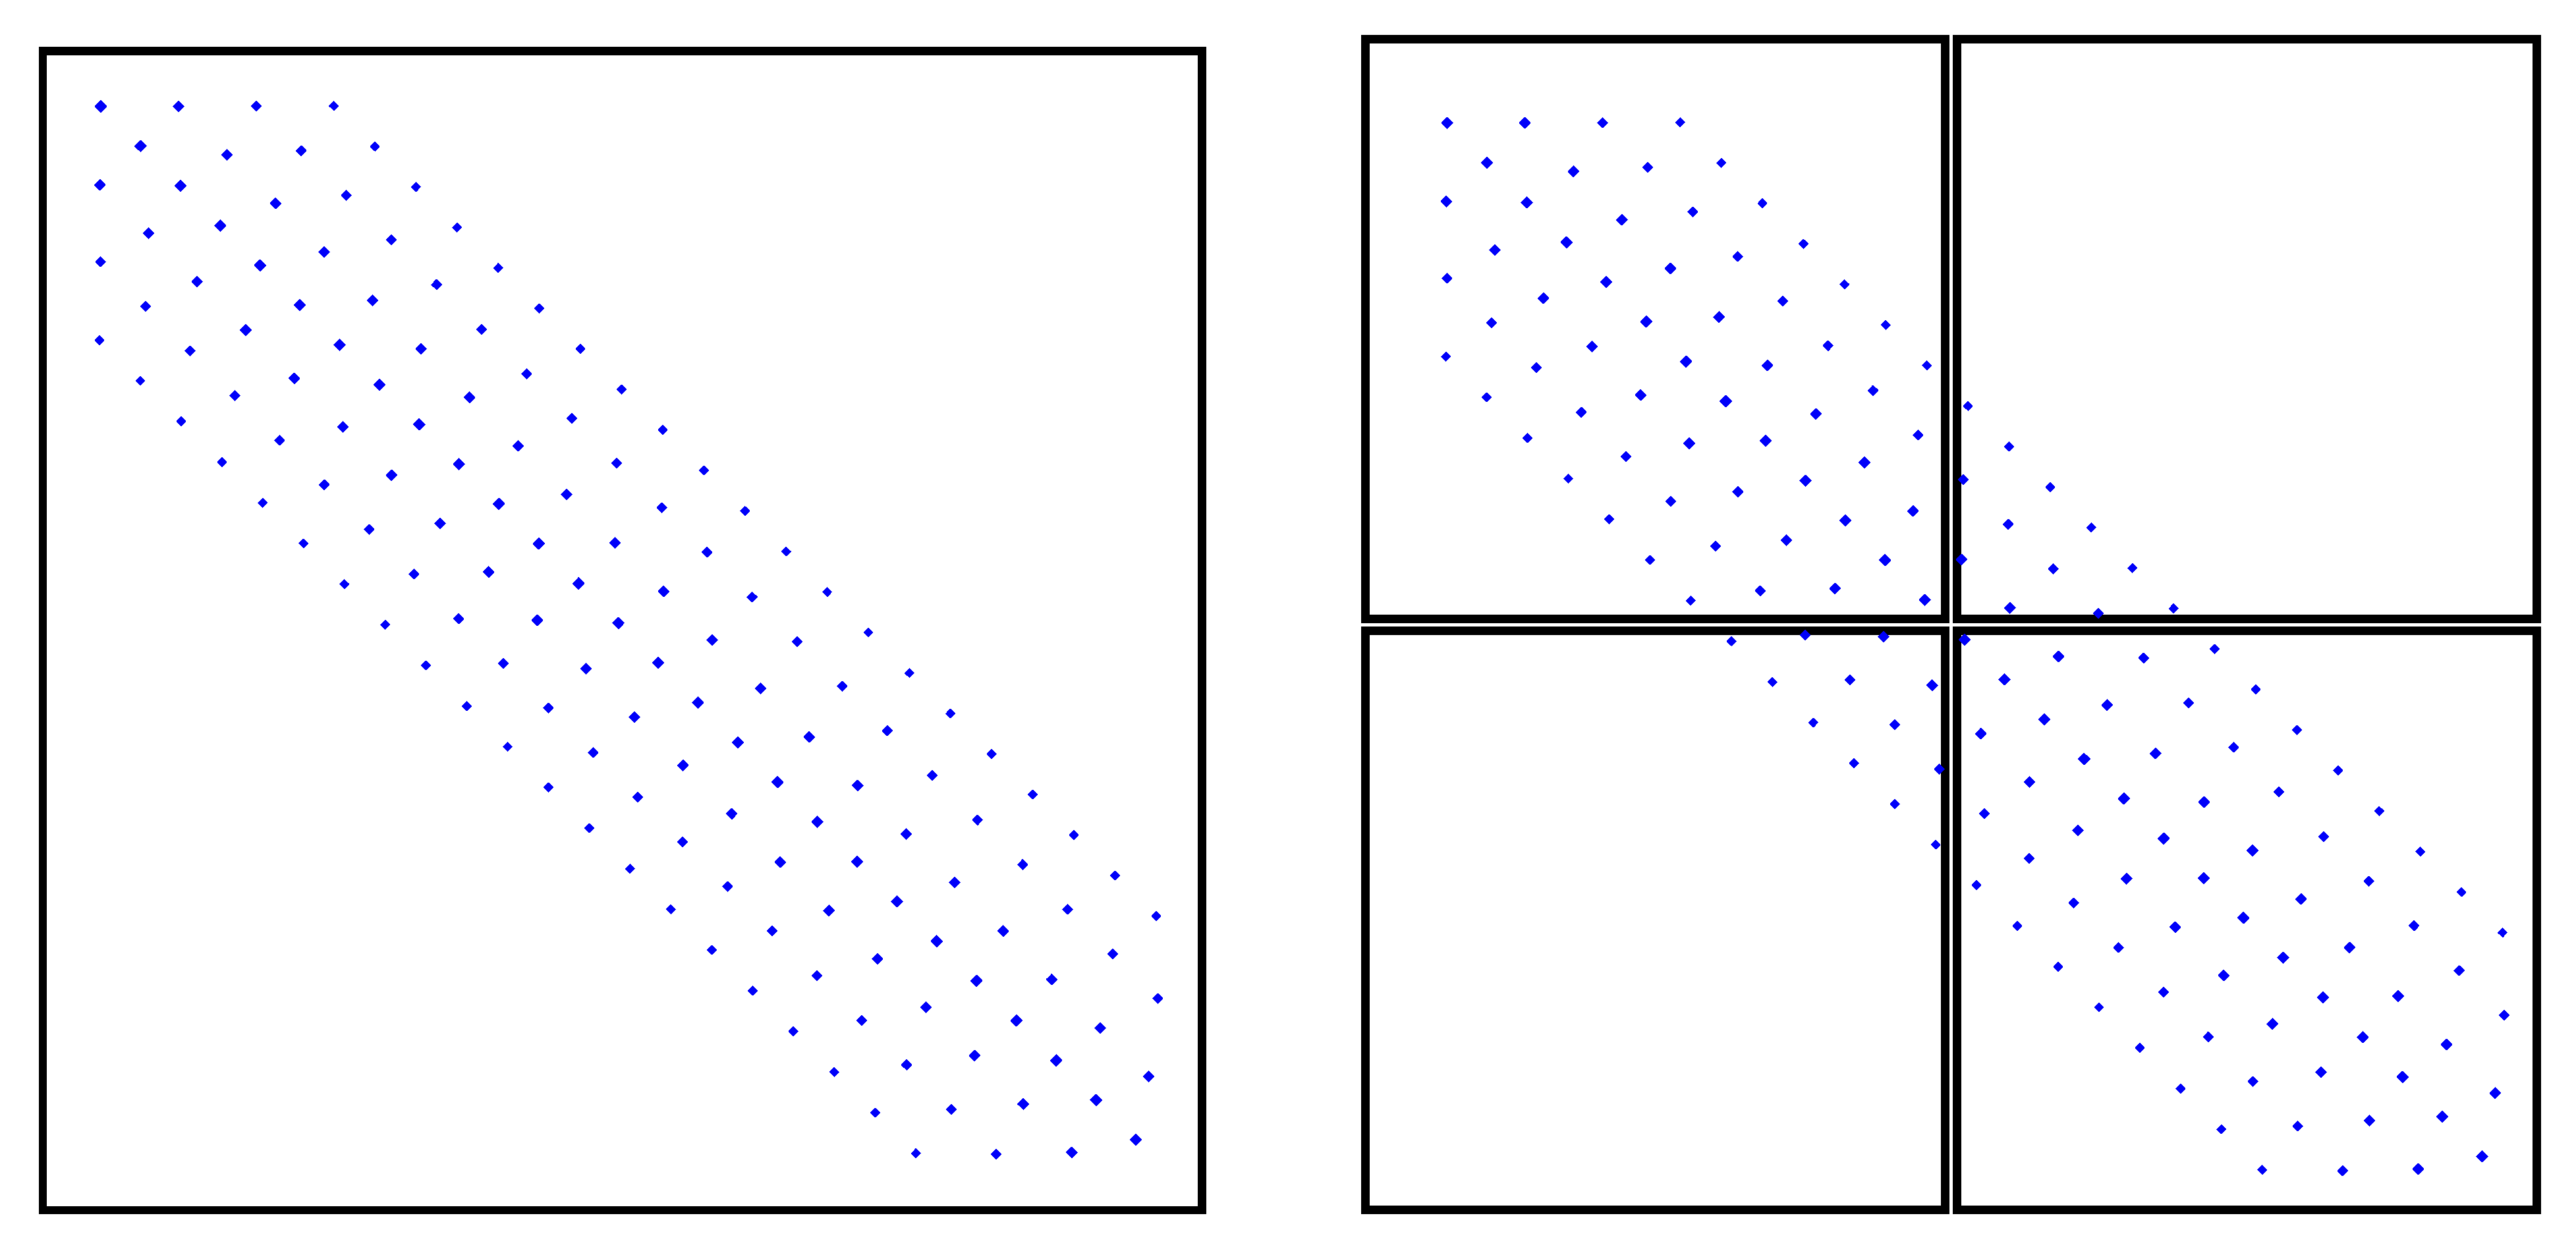
\includegraphics[width=8.5cm,height=4cm]{./figures/split3.pdf}
 \caption{Using row and column sizes to decide when to stop the recursion is not efficient, because the top left block is the same size as the top right one, but it should be divided to more sub-blocks.}
 \label{fig:thres}
\end{figure}

Furthermore, by splitting sparse matrices recursively, we will have more and more zero rows and columns in the resulting blocks. So, using row size and column size of the blocks is not very helpful. Instead, we use nonzero rows and nonzero columns.

At the start of the recursive function, we compute the number of nonzero rows of A ($A\_nnz\_row$) and nonzero columns of B ($B\_nnz\_col$). A threshold for 
\begin{equation}
    \nnzsz := A\_nnz\_row \times B\_nnz\_col\label{eq:thres2}
\end{equation}

is set. Our algorithm has a profiling step where it empirically determines the appropriate threshold by running several test cases. On the machines we used,  $20M$ was chosen as the threshold. We continue splitting the matrices until the threshold is reached, and then we preform the multiplication.

%First method uses a dense matrix.
%The matrices are ordered as column-major.
% In the first method, a dense matrix of size $\nnzsz$ is initialized to $0$. \mr{explain better:}Each nonzero of $B$ is multiplied by its corresponding nonzero of $A$ and the result will be added to the corresponding index in the dense matrix. At the end, we go through the dense matrix and add the nonzeros to the final multiplication matrix.

We have implemented two methods to perform the multiplication: 
\begin{enumerate}
    \item dense buffer
    \item hashmap
\end{enumerate}

When performing the multiplication, at least one of the matrices, typically the output, needs random access as it is accumulating the results. Given that the divide and conquer approach has reduced the size of the output matrix, the first approach is to keep a temporary buffer for dense matrix storage. Each nonzero of $B$ is multiplied by its corresponding nonzero of $A$ and the result will be added to the corresponding index in the dense matrix. As long as the dense matrix is small enough to fit within the L2 cache, we should get good performance. At the end of the multiplication, we traverse the dense matrix and extract the non-zeros as a sparse matrix. This approach works well as long as the resulting matrix is dense. We allocate a memory block of size of the threshold before starting the matrix product. When we reach the stop condition for each recursive call, we preform the following steps:
\begin{enumerate}
    \item Initialize the first \nnzsz~ entries to 0.
    \item Perform the multiplication and add the result entries to the buffer matrix.
    \item Extract nonzeros from the dense matrix and add them to C.
\end{enumerate}

When the ratio of nonzeros to \nnzsz~ is low, it becomes inefficient to traverse the whole dense matrix and check for nonzeros in the final stage. To solve this issue, we use an efficient hashmap to achieve similar results without the $\mathcal{O}(n^2)$ overhead of extracting the non-zeros from the dense matrix. The entry's index is the key and its value is the hashmap's value. When we want to add the multiplication of nonzeros of $A$ and $B$ to the hashmap, we check if the index exists in the map. If it exists the value is being added to the existing one's. Otherwise a new entry will be added to the hashmap. Clearly, there is an overhead to this approach that needs to be balanced against the overheads associated with the dense representation. 

To measure the effectiveness of our method in a practical situation, we have implemented the \recmm~ function in our Algebraic Multigrid solver, called \textit{Saena}, and performed \textsc{GEMM} twice to compute the coarse matrix of the 3D Poisson Problem.

In Figure~\ref{fig:lap60}, we compare the two methods for computing coarse matrix $Ac = R \times A \times P$, in which $A$ is the 3D Poisson problem of size $216k$. For $0 \leq \nnzsz \leq 10M$, in $1M$ steps, we compare the two methods in order to develop an efficient hybrid algorithm. For instance, the first point indicates that the dense structure is better than the hashmap approach in $1245$ cases for the multiplications such that $0 \le\ \nnzsz < 1M$. For the lower range the dense representation is better and for the higher range the hashmap is significantly faster. Figure~\ref{fig:eco} shows the same experiment for matrix ID $1882$ from SuiteSparse (Florida) Matrix Collection, which is a sparse matrix of size $1M$ and $5M$ nonzero.

\begin{figure*}[p]
 \centering
 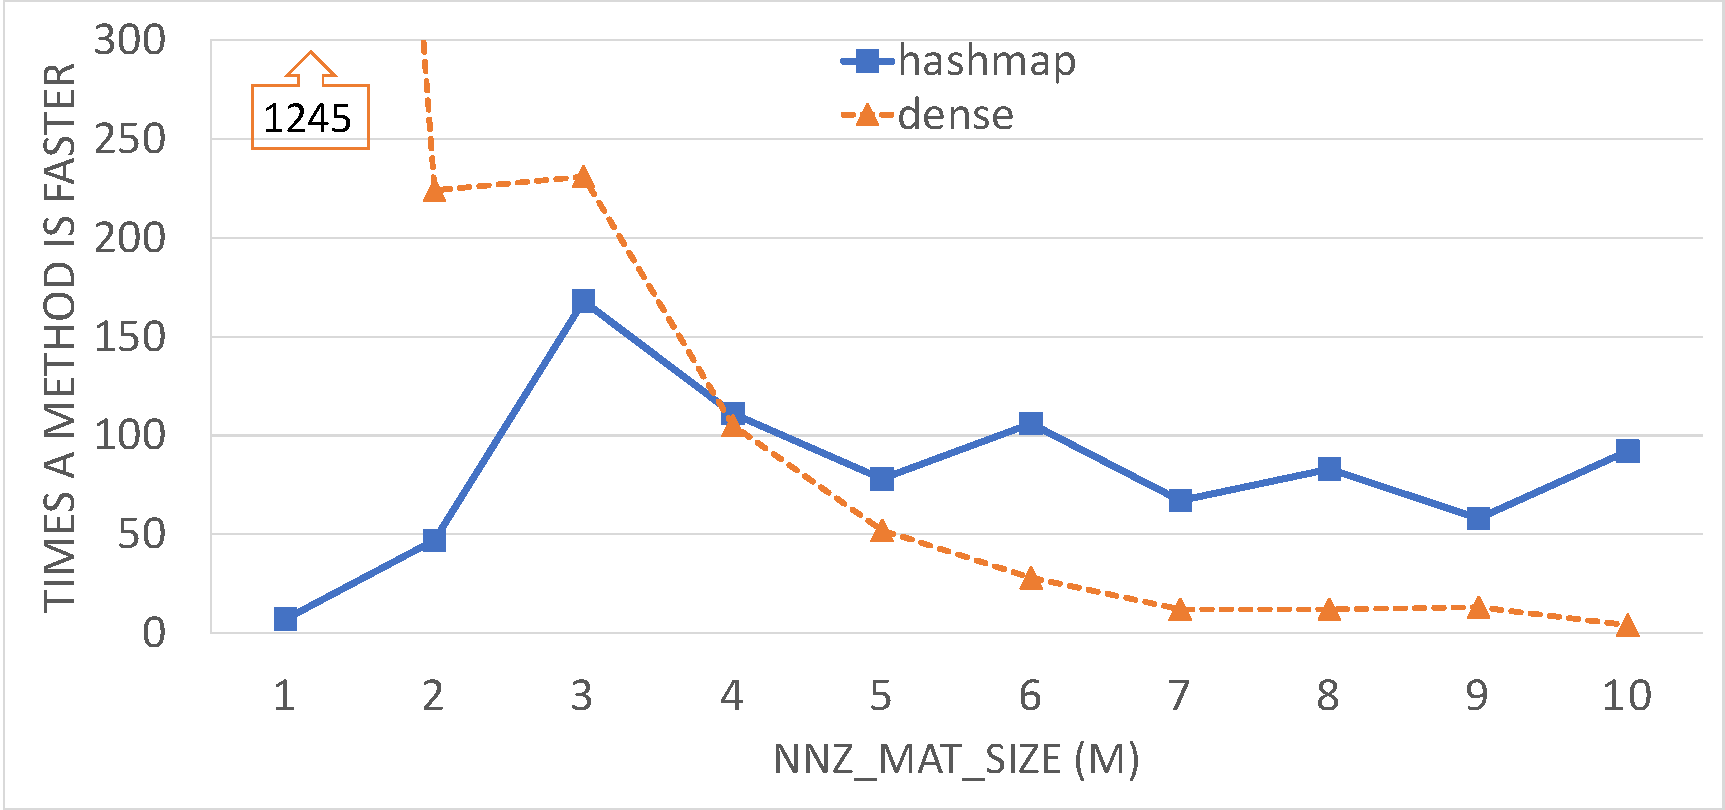
\includegraphics[width=11.8cm,height=5.4cm]{./figures/lap60_range.pdf}
 \caption{Comparison between dense structure method with hashmap to compute coarse matrix $Ac = R \times A \times P$, in which $A$ is the 3D Poisson problem of size $216k$. The plot shows the number of times each method is faster than the other one in intervals of $1M$ for $\nnzsz$.}
 \label{fig:lap60}
\end{figure*}

A combination of these two methods would give us the best performance across different matrix structures and densities. The dense method is being used for the lower range and the hashmap for the higher range.
We have done a series of experiments to determine the threshold when to switch between the two methods. Figures~\ref{fig:lap60} and \ref{fig:eco} suggest to use the dense structure method when $0 \le\ \nnzsz < 4M$ and use hashmap for the rest. We noticed that when hashmaps are better, the difference time between the two methods on average is higher. In other words, on average, $n$ times performing hashmap is faster than $n$ times using the dense structure. So empirically, we found $1M$ to be a good estimate for switching between the two methods.

\begin{figure*}[p]
 \centering
 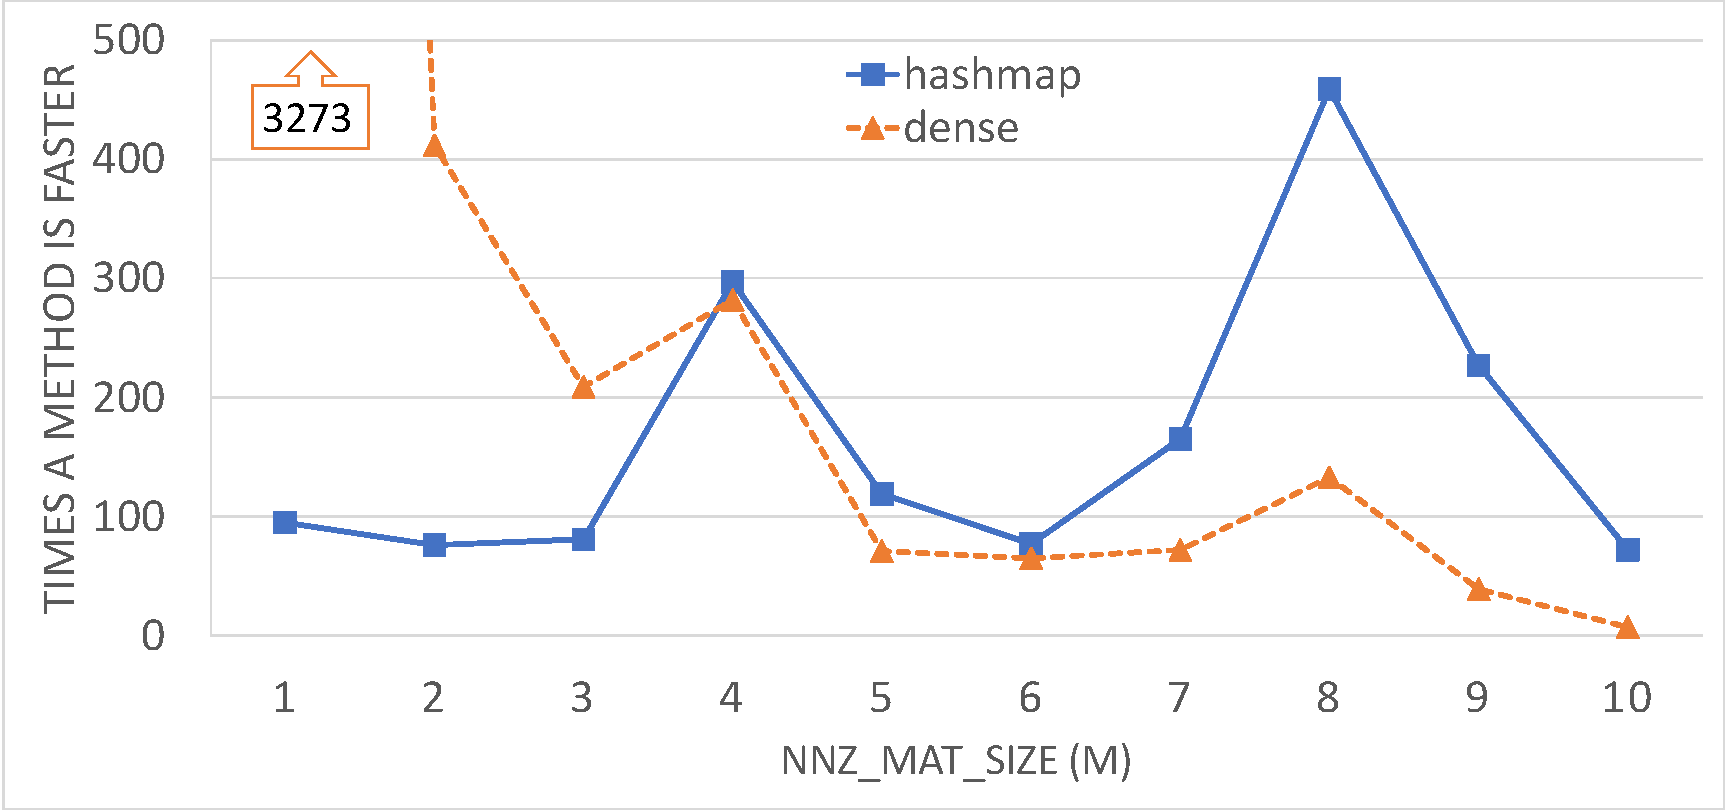
\includegraphics[width=11.8cm,height=5.4cm]{./figures/eco_range.pdf}
 \caption{Comparison between dense structure method with hashmap to compute coarse matrix $Ac = R \times A \times P$, in which $A$ is matrix ID $1882$ from SuiteSparse (Florida) Matrix Collection. The plot shows the number of times each method is faster than the other one in intervals of $1M$ for $\nnzsz$.}
 \label{fig:eco}
\end{figure*}

\begin{figure*}[p]
 \centering
 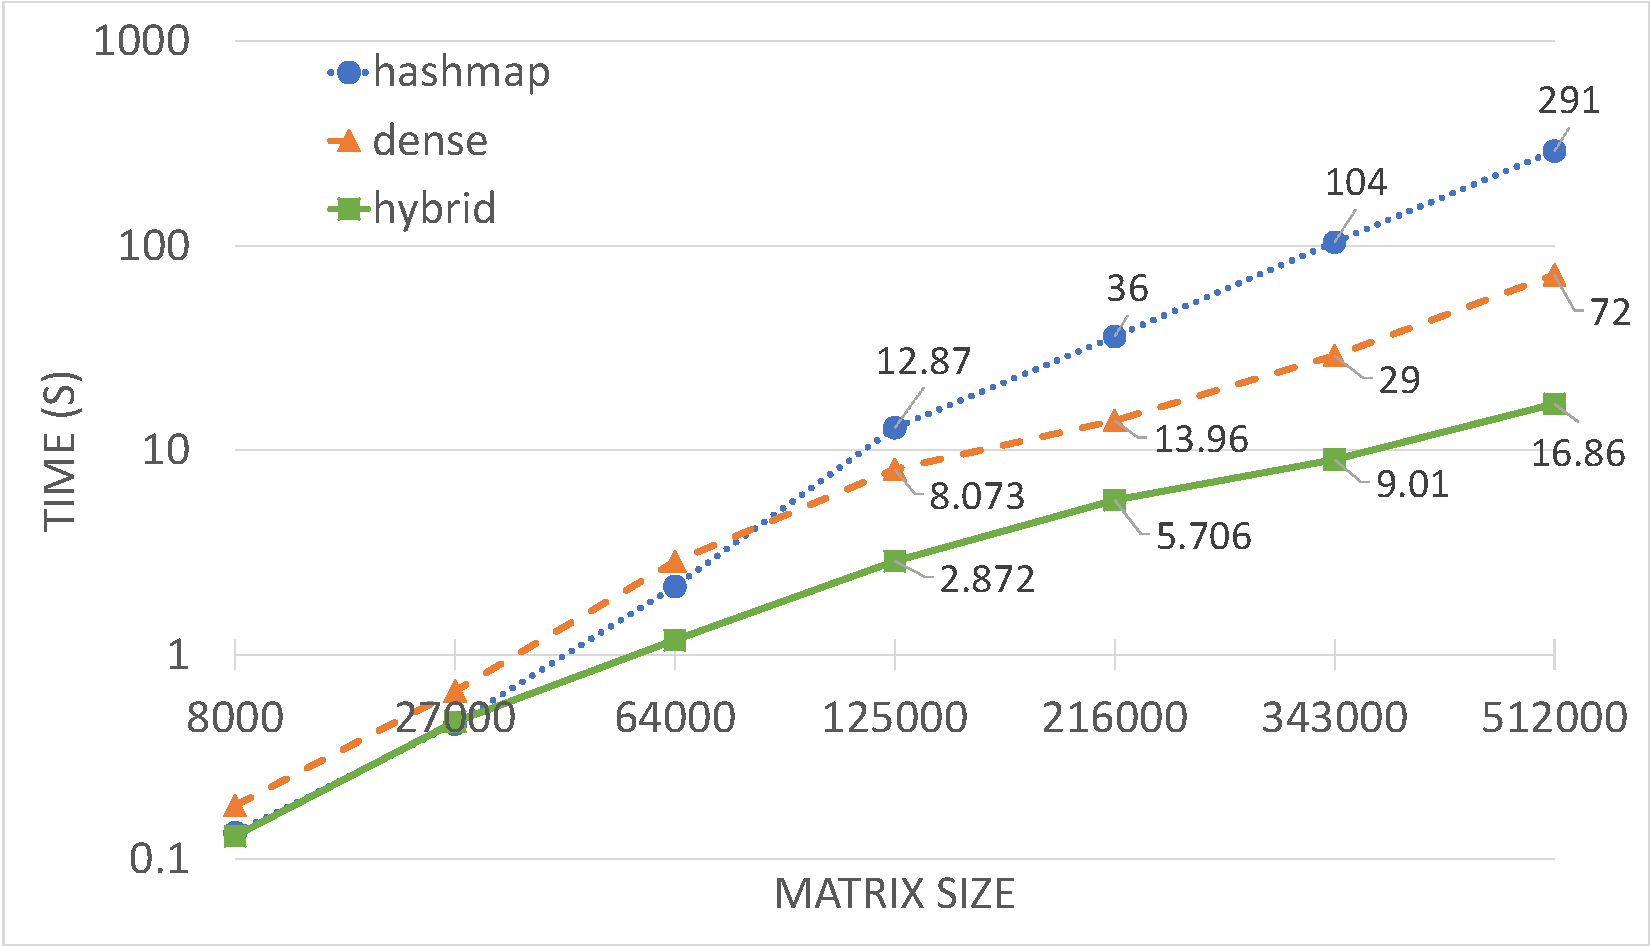
\includegraphics[width=11.8cm,height=6.9cm]{./figures/mix.pdf}
 \caption{Comparison between the three methods to do Case 1: only using hashmap, only using the dense structure, and the hybrid method. They are used in Case 1 part of \recmm~ to compute the first coarse matrix (the triple multiplication) of 7 matrices (3D Poisson) of different sizes.}
 \label{fig:mix}
\end{figure*}

Figure~\ref{fig:mix} compares the hybrid method with the basic two methods. We have compared the three approaches on different sizes of 3D Poisson problem, ranging from $8k$ to almost half a million. For instance, for the case where the matrix is of size $512k$, performing the triple matrix product takes $291s$ if only hashmap is used for Case 1, takes $72s$ if only the dense structure is used and finally takes almost $17s$ when the hybrid approach is utilized.


\subsubsection{Case 2}
\label{sec:case2}
When A is horizontal, i.e. its row size is less than or equal to its column size, we halve A by column based on its column size (Figure~\ref{fig:case2_left}). Since row size of B equals column size of A, we halve B by row, so it will be a split similar to A, but horizontally.
Then, the \recmm~ will be called twice, once on $A1$ and $B1$, and again on $A2$ and $B2$ (Algorithm~\ref{alg:case2}). The results of the two multiplications need to be added together at the end. It means, there will be entries for the result matrix with the same index. We call these entries \textit{duplicates}. Since there will be numerous nested recursive calls, we avoid doing adding duplicates at this stage. After the starting recursive function is finished, we sort $C$ and then add the duplicates only once at the end.

\begin{figure}[tbh]
    \centering
    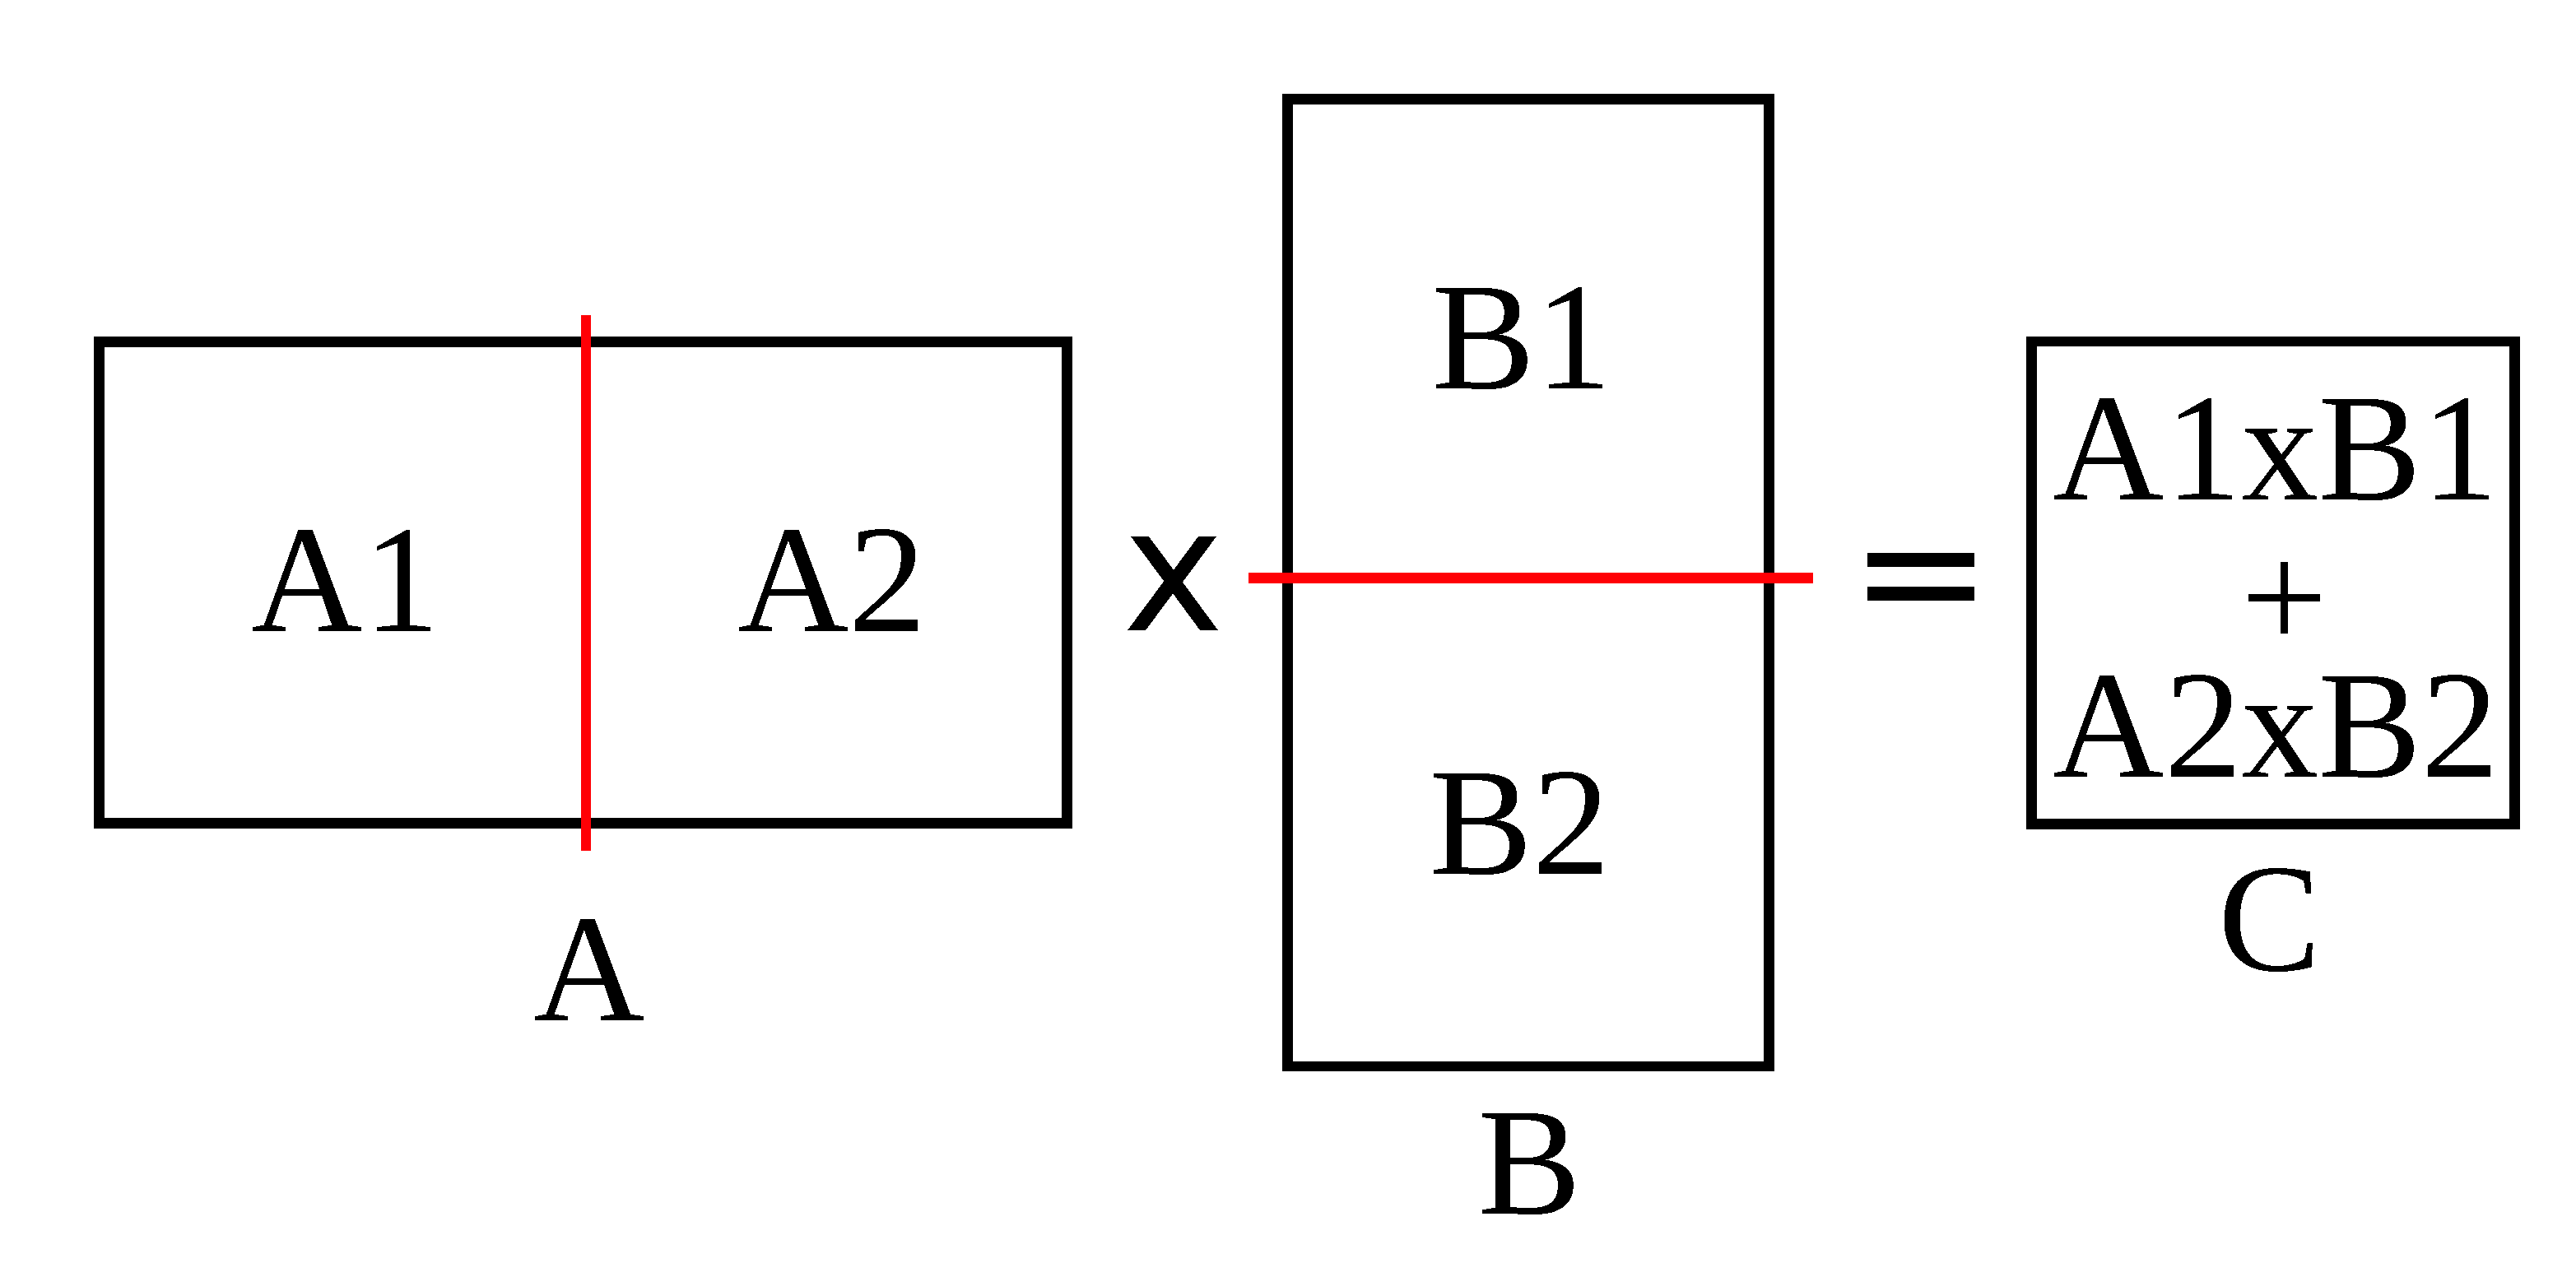
\includegraphics[width=7cm,height=3.1cm]{./figures/case2_001.pdf}
    \caption{Case 2: When A is horizontal, split A by column and B by row. Call the recursive function twice.}
    \label{fig:case2_left}
\end{figure}

\begin{figure}[tbh]
    \centering
    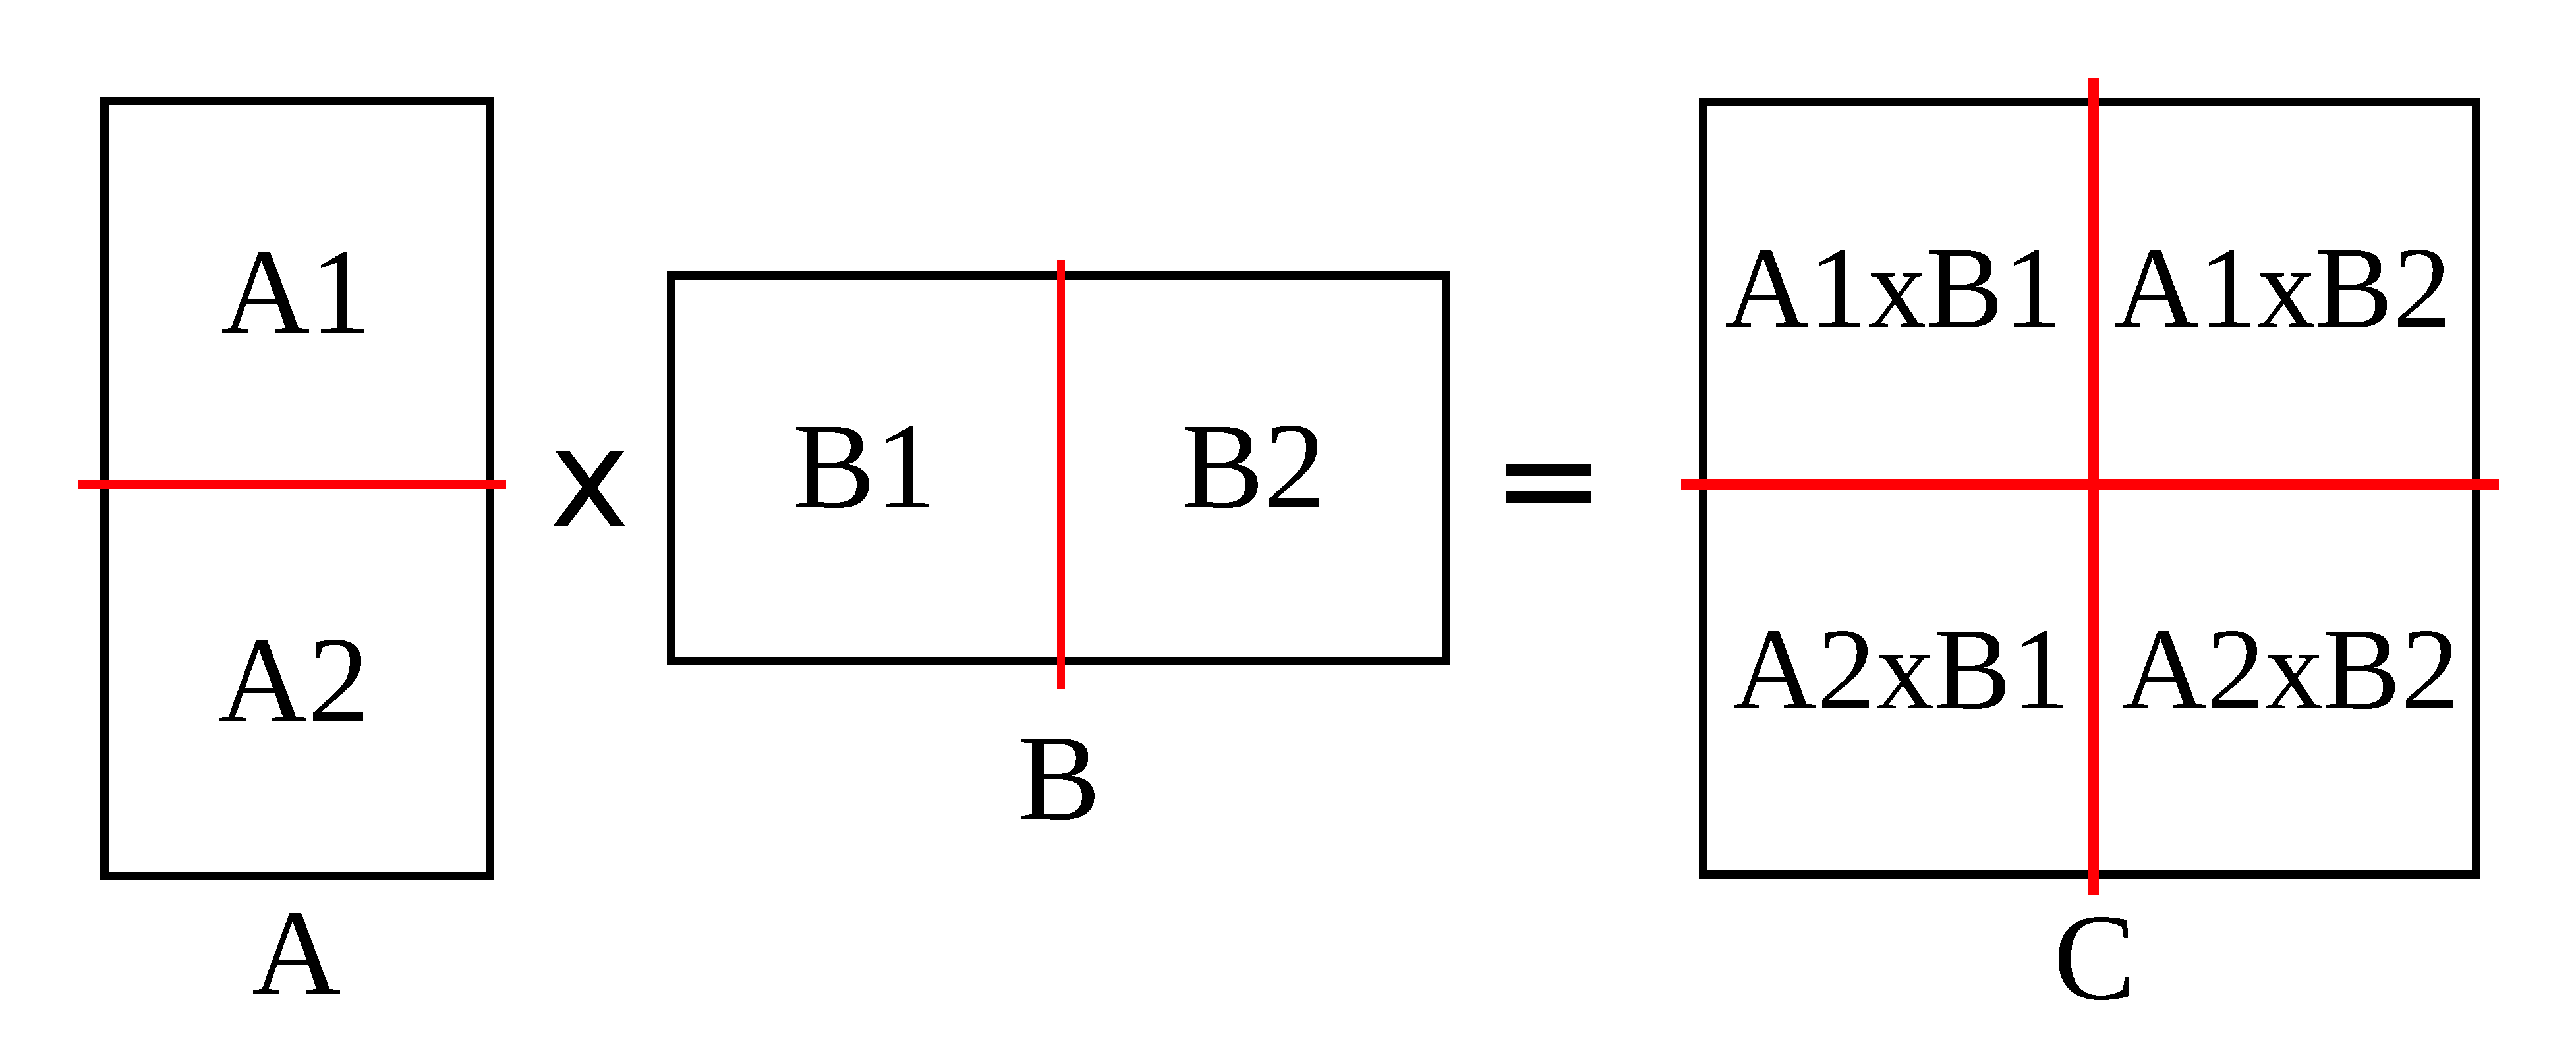
\includegraphics[width=7.9cm,height=3.1cm]{./figures/case3_001.pdf}
    \caption{Case 3: When A is vertical, split A by row and B by column. Call the recursive function four times.}
    \label{fig:case3}
\end{figure}

\begin{algorithm}[tbh] 
  %\footnotesize
  \caption{Case 2: $C = \recmm2(A, B)$} 
  \begin{algorithmic}[1]
    \Require $A$, $B$
    \Ensure  $C$
    \State $(A1, A2) = \spc(A)$
    \State $(B1, B2) = \spr(B)$
    \State $C \leftarrow \recmm(A1,B1)$
    \State $C \leftarrow \recmm(A2,B2)$
    %\State $C \leftarrow \textsc{mergesort}(C1, C2)$
  \end{algorithmic}
  \label{alg:case2}
\end{algorithm}


\subsubsection{Case 3}
\label{sec:case3}
When A is vertical, i.e. its row size is greater than its column size, we halve A by row and B by column (Figure~\ref{fig:case3}). This time the \recmm~ will be called four times (Algorithm~\ref{alg:case3}).  Although we have 4 recursive calls in this case, but there is no duplicates at the end, which makes this case more efficient than Case 2 for the total time, because we have a smaller set of entries to sort and add the duplicates.

\iffalse
\begin{figure}[tbh]
 \centering
 %\Description{Description}
 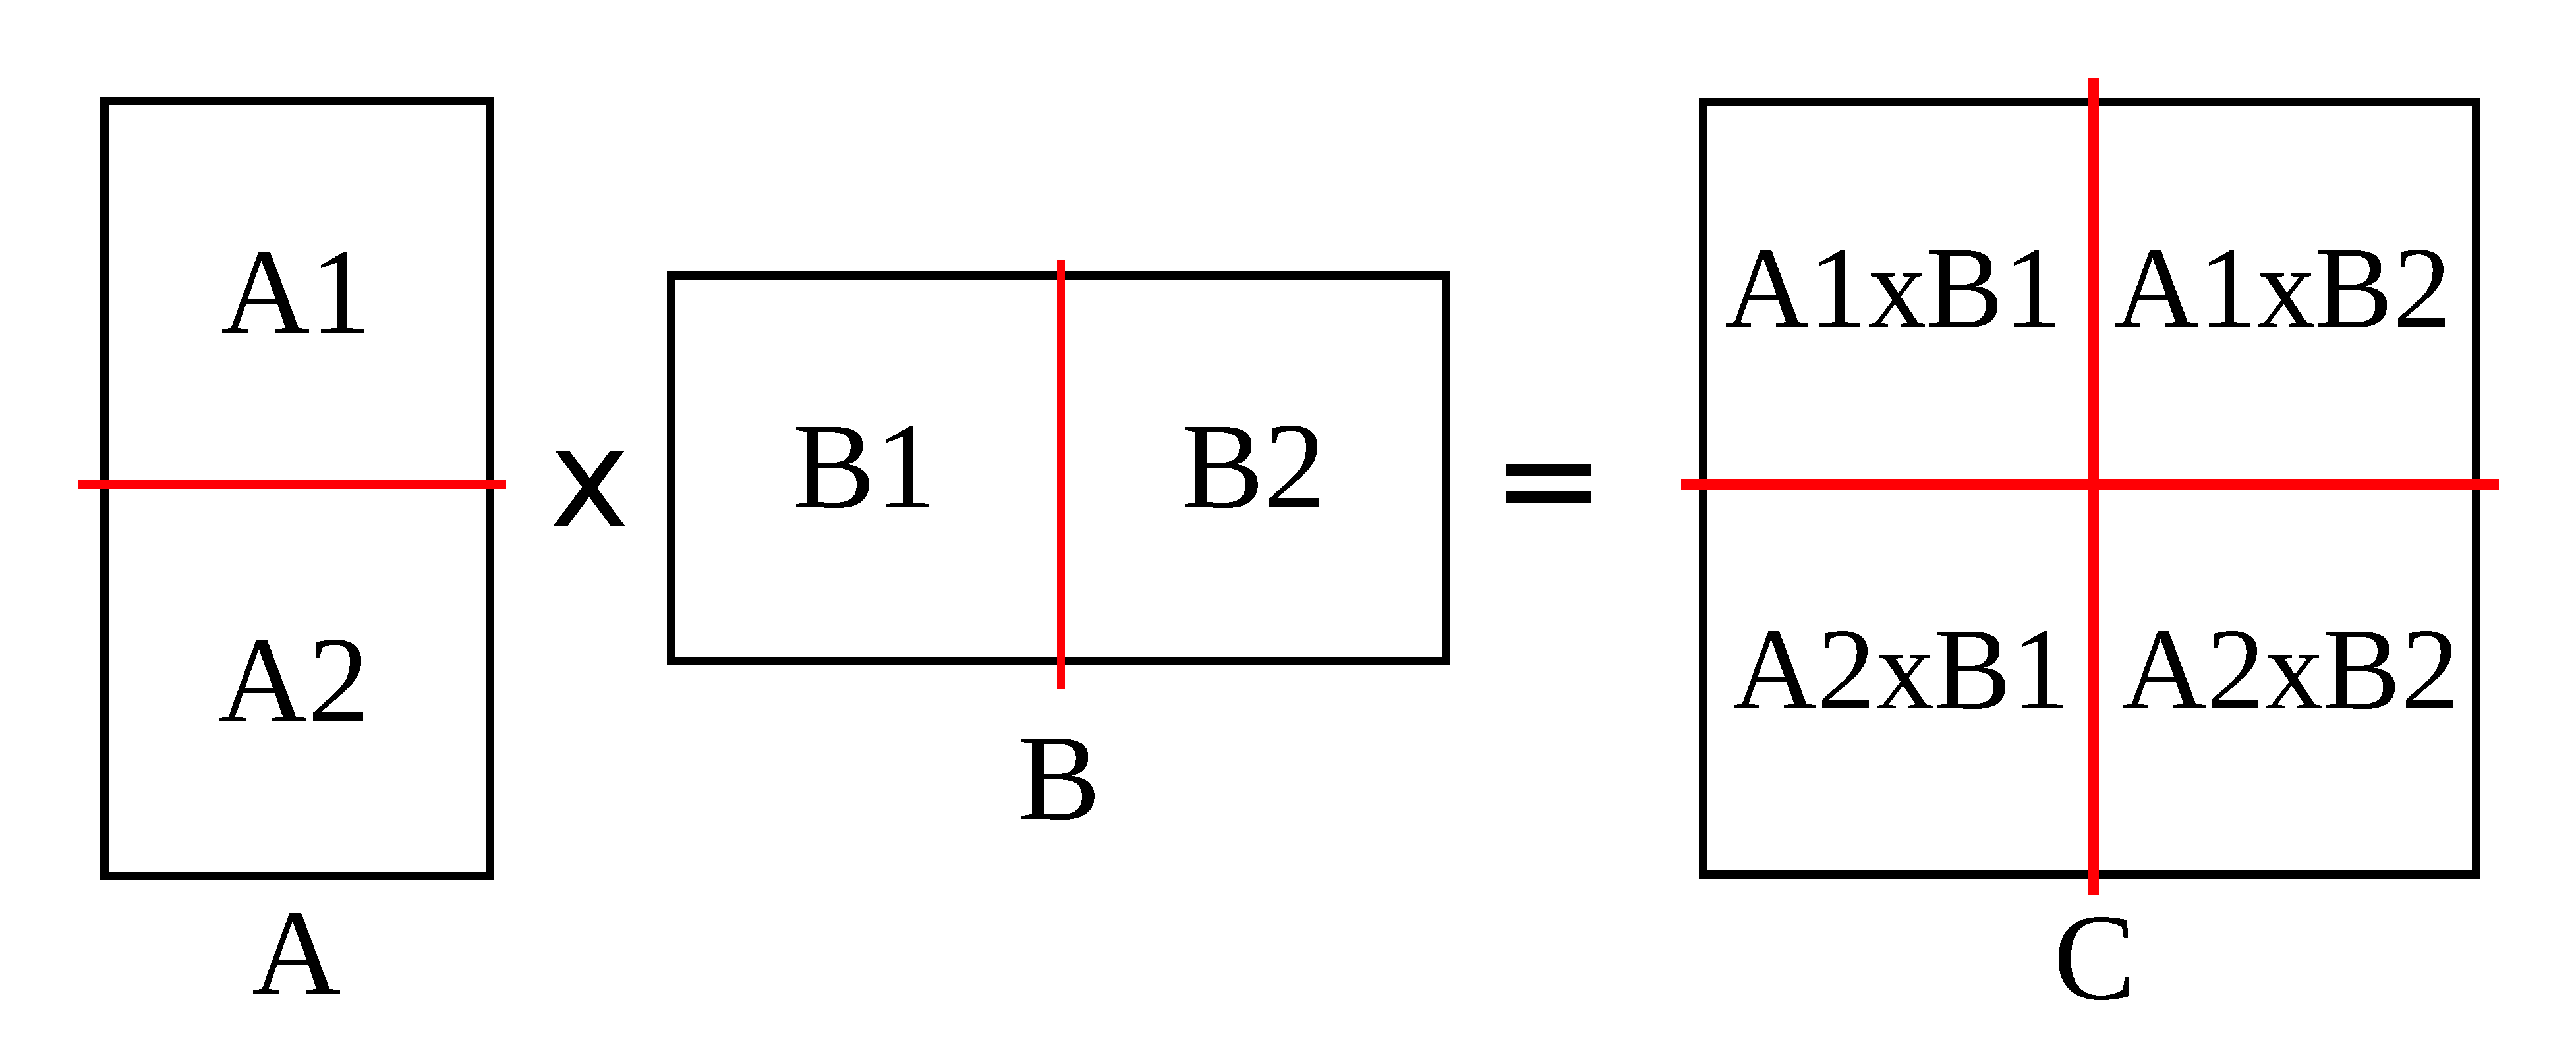
\includegraphics[width=6cm,height=2.5cm]{./figures/case3_001.pdf}
 \caption{Case 3: When A is vertical, split A by row and B by column. Call the recursive function four times.}
 \label{fig:case3}
\end{figure}
\fi

\begin{algorithm}[H] 
  %\footnotesize
  \caption{Case 3: $C = \recmm3(A, B)$}
  \begin{algorithmic}[1]
    \Require $A$, $B$
    \Ensure  $C$
    \State $(A1, A2) = \spr(A)$
    \State $(B1, B2) = \spc(B)$
    \State $C \leftarrow \recmm(A1,B1)$
    \State $C \leftarrow \recmm(A2,B1)$
    \State $C \leftarrow \recmm(A1,B2)$
    \State $C \leftarrow \recmm(A2,B2)$
    %\State $\textsc{sort}(C)$
  \end{algorithmic}
  \label{alg:case3}
\end{algorithm}

We have also implemented splitting based on the number of nonzeros. In \textit{Case 2}, we split $A$ in a way to have half of nonzeros in $A1$, and the other half in $A2$. The same split is used for $B$. In \textit{Case 3}, we do the same, but separately for both $A$ and $B$. We compare these two splitting methods in the last section.

\subsubsection{All together}

When all three cases work together, we have Case 2 and Case 3, that aim to divide the matrices into skinny matrices such that the resulting matrix is small. Then by using a hybrid multiplication algorithm, we get these results. These results are then accumulated and merged together. From a memory access perspective, the accumulation and merging required for Case 2 and 3 is structured access to the matrix, with the only random access happening during Case 1. This makes the overall algorithm very efficient. 

\subsection{Communication}
\label{sec:amg}

In the previous section we explained how to perform \recmm~ if the data is available locally. In this section, we explain how the communication is done to perform
\begin{equation}
    C = A \times B
\end{equation}
in a distributed fashion for general (non necessarily symmetric) matrices $A$ and $B$. Also, we propose a method to improve the performance and scalability of \recmm~ if $B$ is symmetric.

Matrices are partitioned across multiple processors by row blocks (Figure~\ref{fig:partition}). Since matrices $A$ and $B$ may have different number of rows, they may not be partitioned the same way. We avoid communicating $A$ in our method and only communicate $B$, to avoid any communication at the end of the multiplication. Algorithm~\ref{alg:comm1} shows how the communication is done. It is an overlapped implementation, so while the processors are communicating the data, the multiplication is being executed on the available data from the previous processor (so executing \recmm~ between the \textit{Isend-Irecv} part and \textit{wait}). This way we save a portion of the time that the communication takes and use it to do the multiplication. The other advantage of our communication algorithm is having each processor to communicate only with their neighbors.

\begin{figure}[tbh]
 \centering
 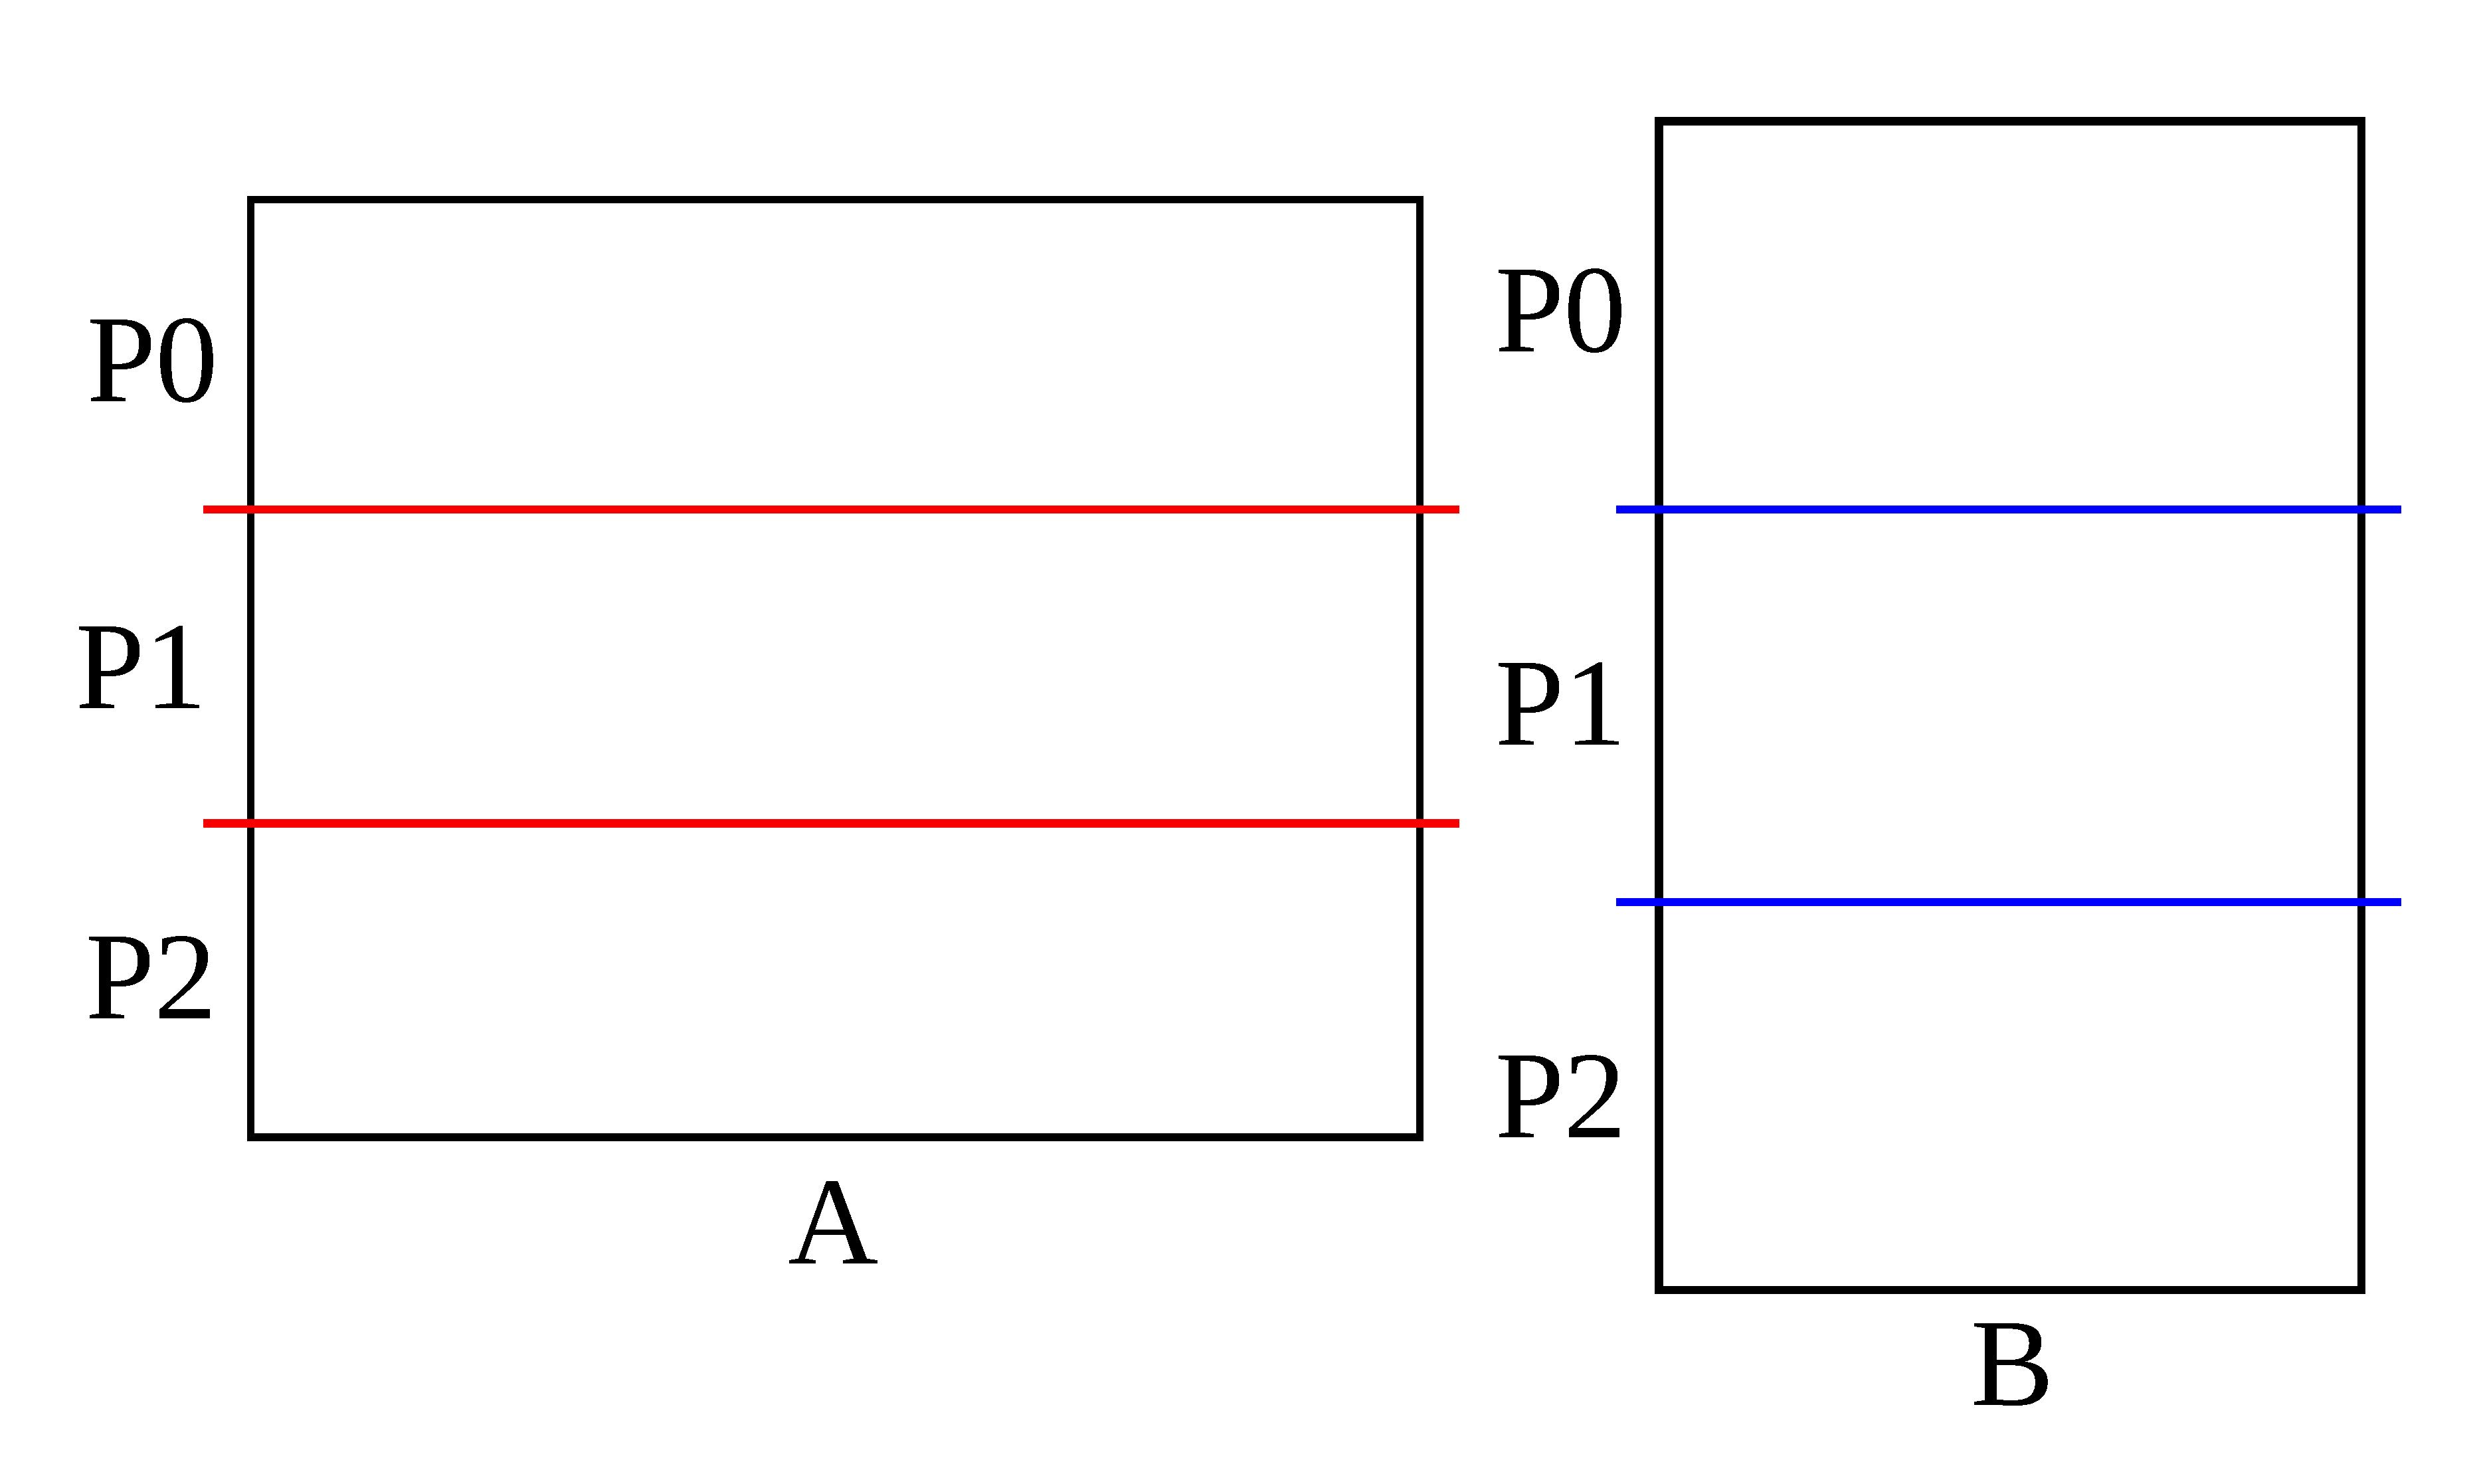
\includegraphics[width=7.8cm,height=4.4cm]{./figures/partition2.pdf}
 \caption{Partitioning of the matrices across the processors in row blocks.}
 \label{fig:partition}
\end{figure}

\begin{algorithm}[H] 
  %\footnotesize
  \caption{$C_i = A_i \times B$}
  \begin{algorithmic}[1]
    \Require $A_i$, $B$
    \Ensure  $C_i$ (result of $A_i \times B$)
    \State $B\_send \leftarrow B_i$
    \For{$k=myrank:myrank+nprocs$}
      \State $Isend(B\_send)$ to left neighbor
      \State $B\_recv \leftarrow$ Irecv(remote $B$) from right neighbor
      \State $C_{i} \leftarrow \recmm(A_i, B\_send)$ 
      \State wait for Isend and Irecv to finish
      \State $swap\_pointers(B\_send,B\_recv)$
    \EndFor
    \State locally sort $C_i$ and add duplicates
  \end{algorithmic}
  \label{alg:comm1} 
\end{algorithm}

Now, we explain how to improve our algorithm to compute $A \times B$, when $B$ is symmetric. Since the number of columns of $A$ equals the number of rows of $B$ (to be able to multiply them), we assume the same division of rows of $B$ on $A$'s columns (blue lines), only to show corresponding parts of $A$ and $B$ that should be multiplied. To compute entry $C_{ij}$, we need to multiply row $i$ of $A$ with column $j$ of $B$ and add them together.
For that, the blocks of $A$ and $B$ with the same color in Figure~\ref{fig:partition3} should be multiplied, and only after multiplying all those blocks we have all the duplicates to add together and have the final value for entry $C_{ij}$ (Line $9$ in Algorithm~\ref{alg:comm1}).

\begin{figure}[tbh]
    \centering
    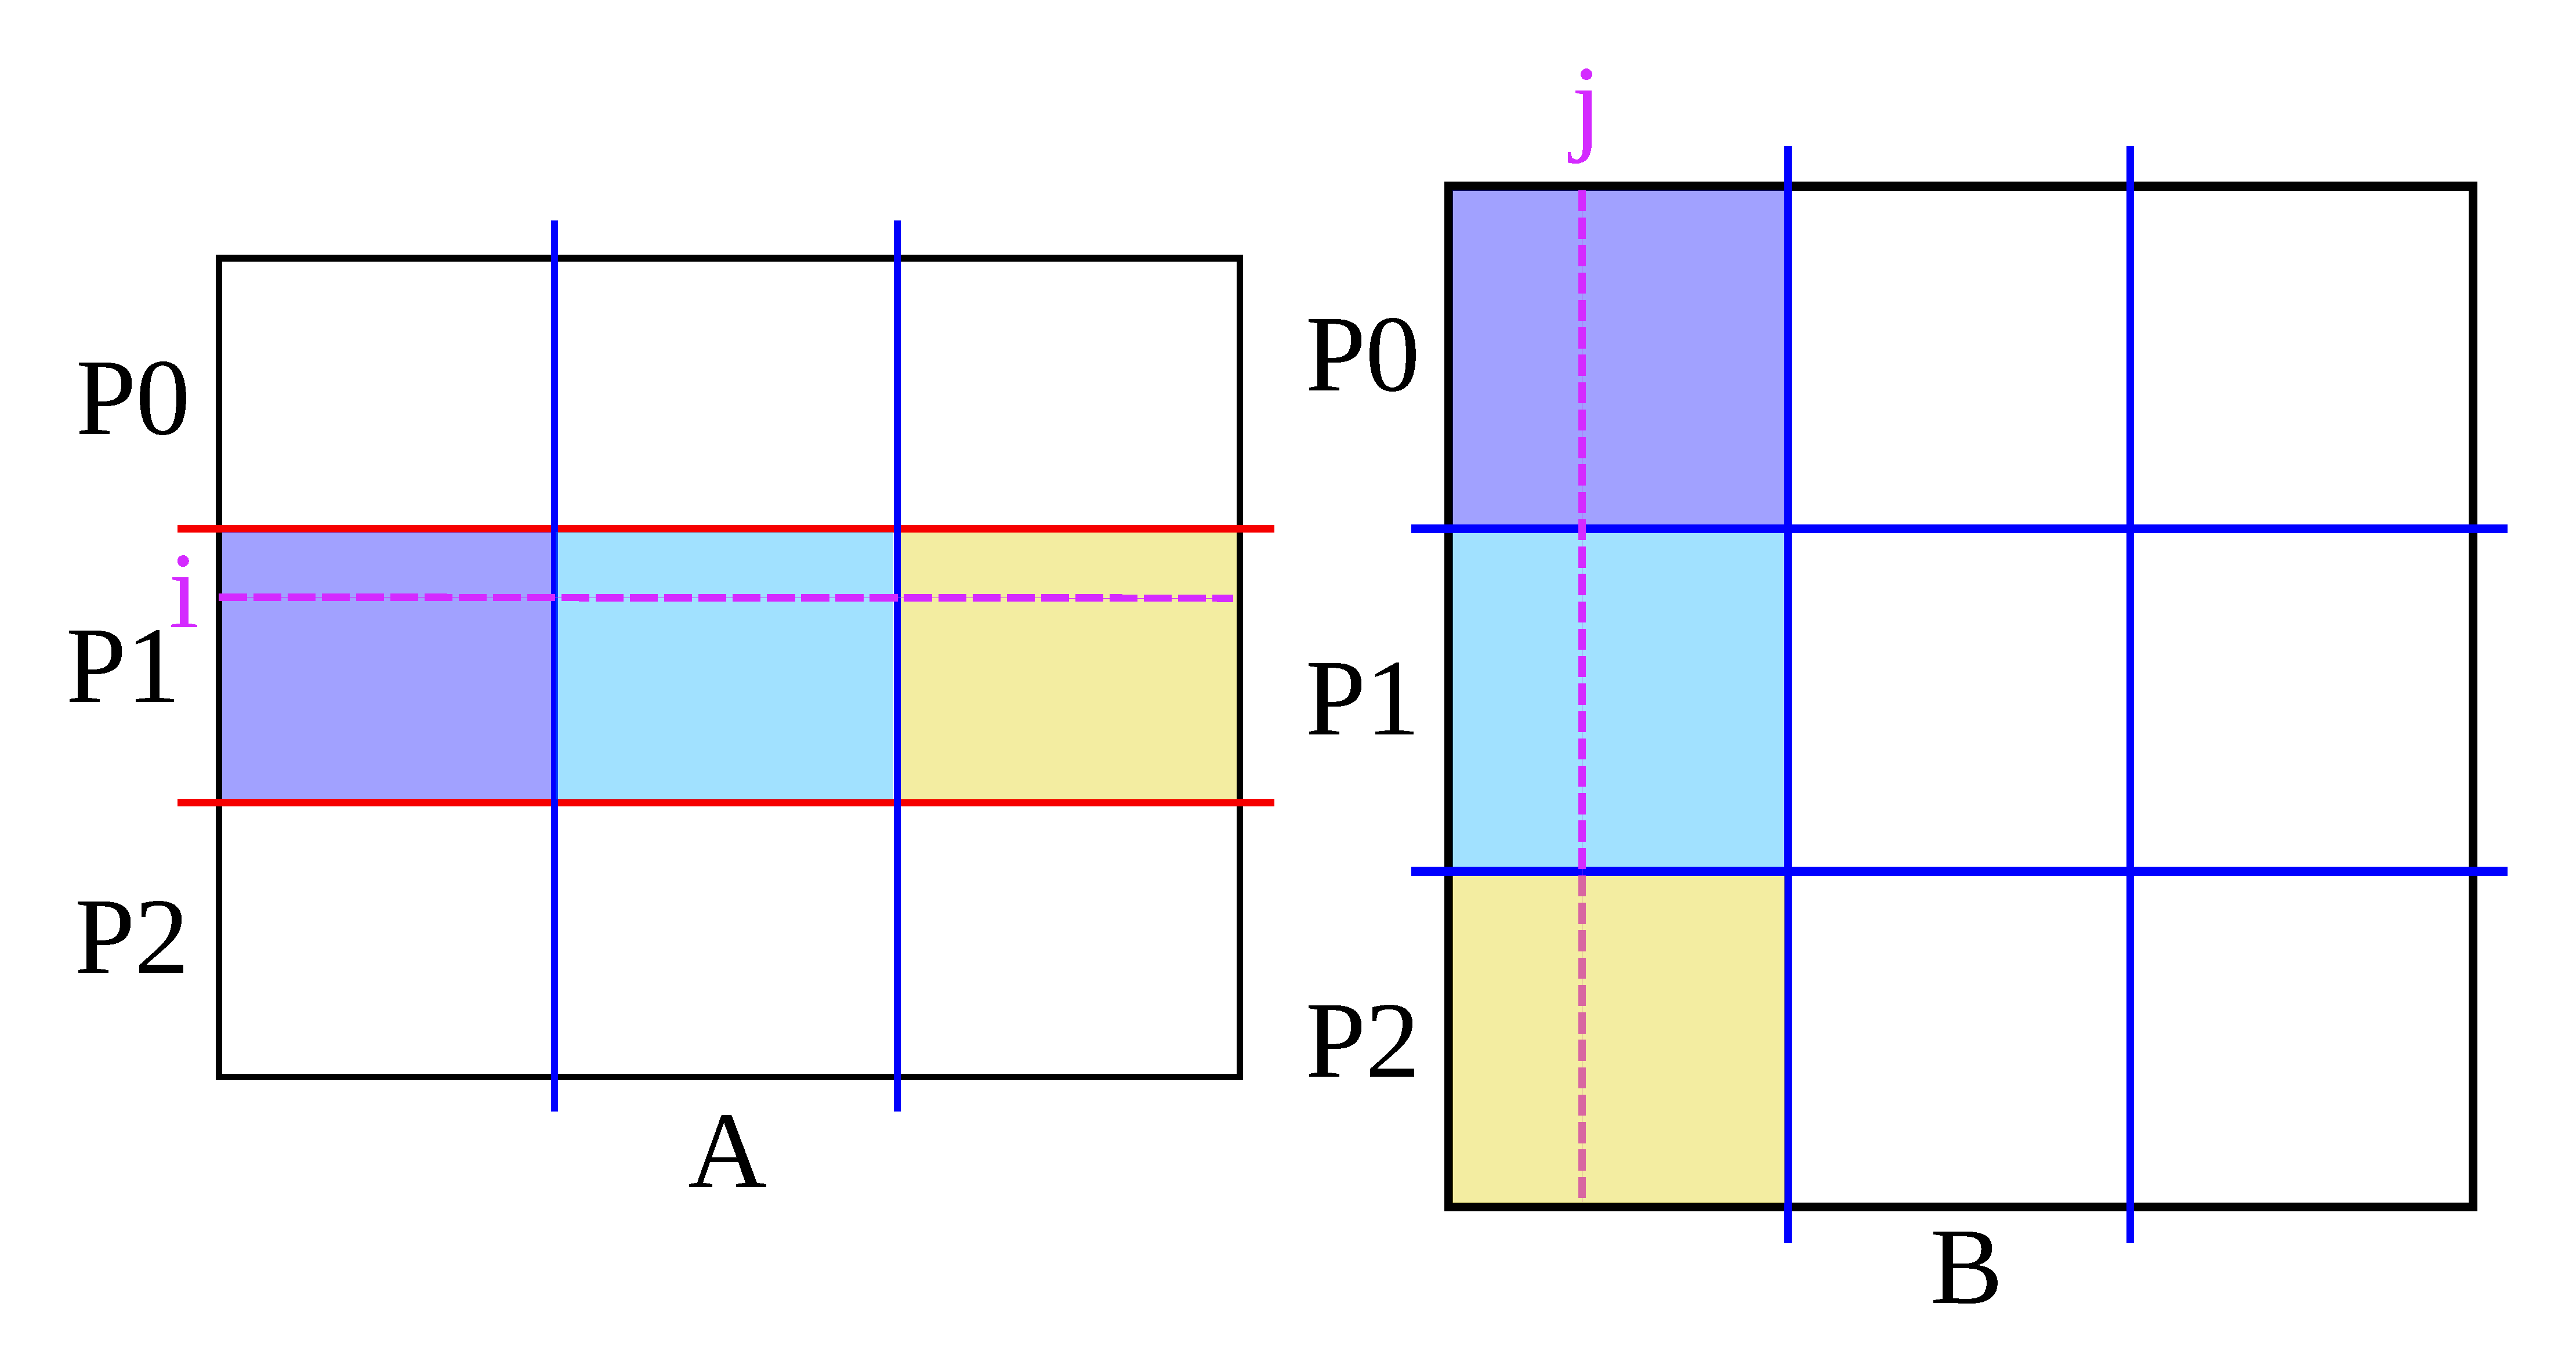
\includegraphics[width=8.4cm,height=4.6cm]{./figures/partition3.pdf}
    \caption{Column $j$ of $B$ is stored on different processors, so to compute entry $C_{ij}$ we need to multiply the parts of $A$ and $B$ with the same color.}
    \label{fig:partition3}
\end{figure}

When $B$ is symmetric, instead of working with $B_i$'s, we consider their local transpose $BT_i$ in Figure~\ref{fig:partition4}.

\begin{figure}[tbh]
    \centering
    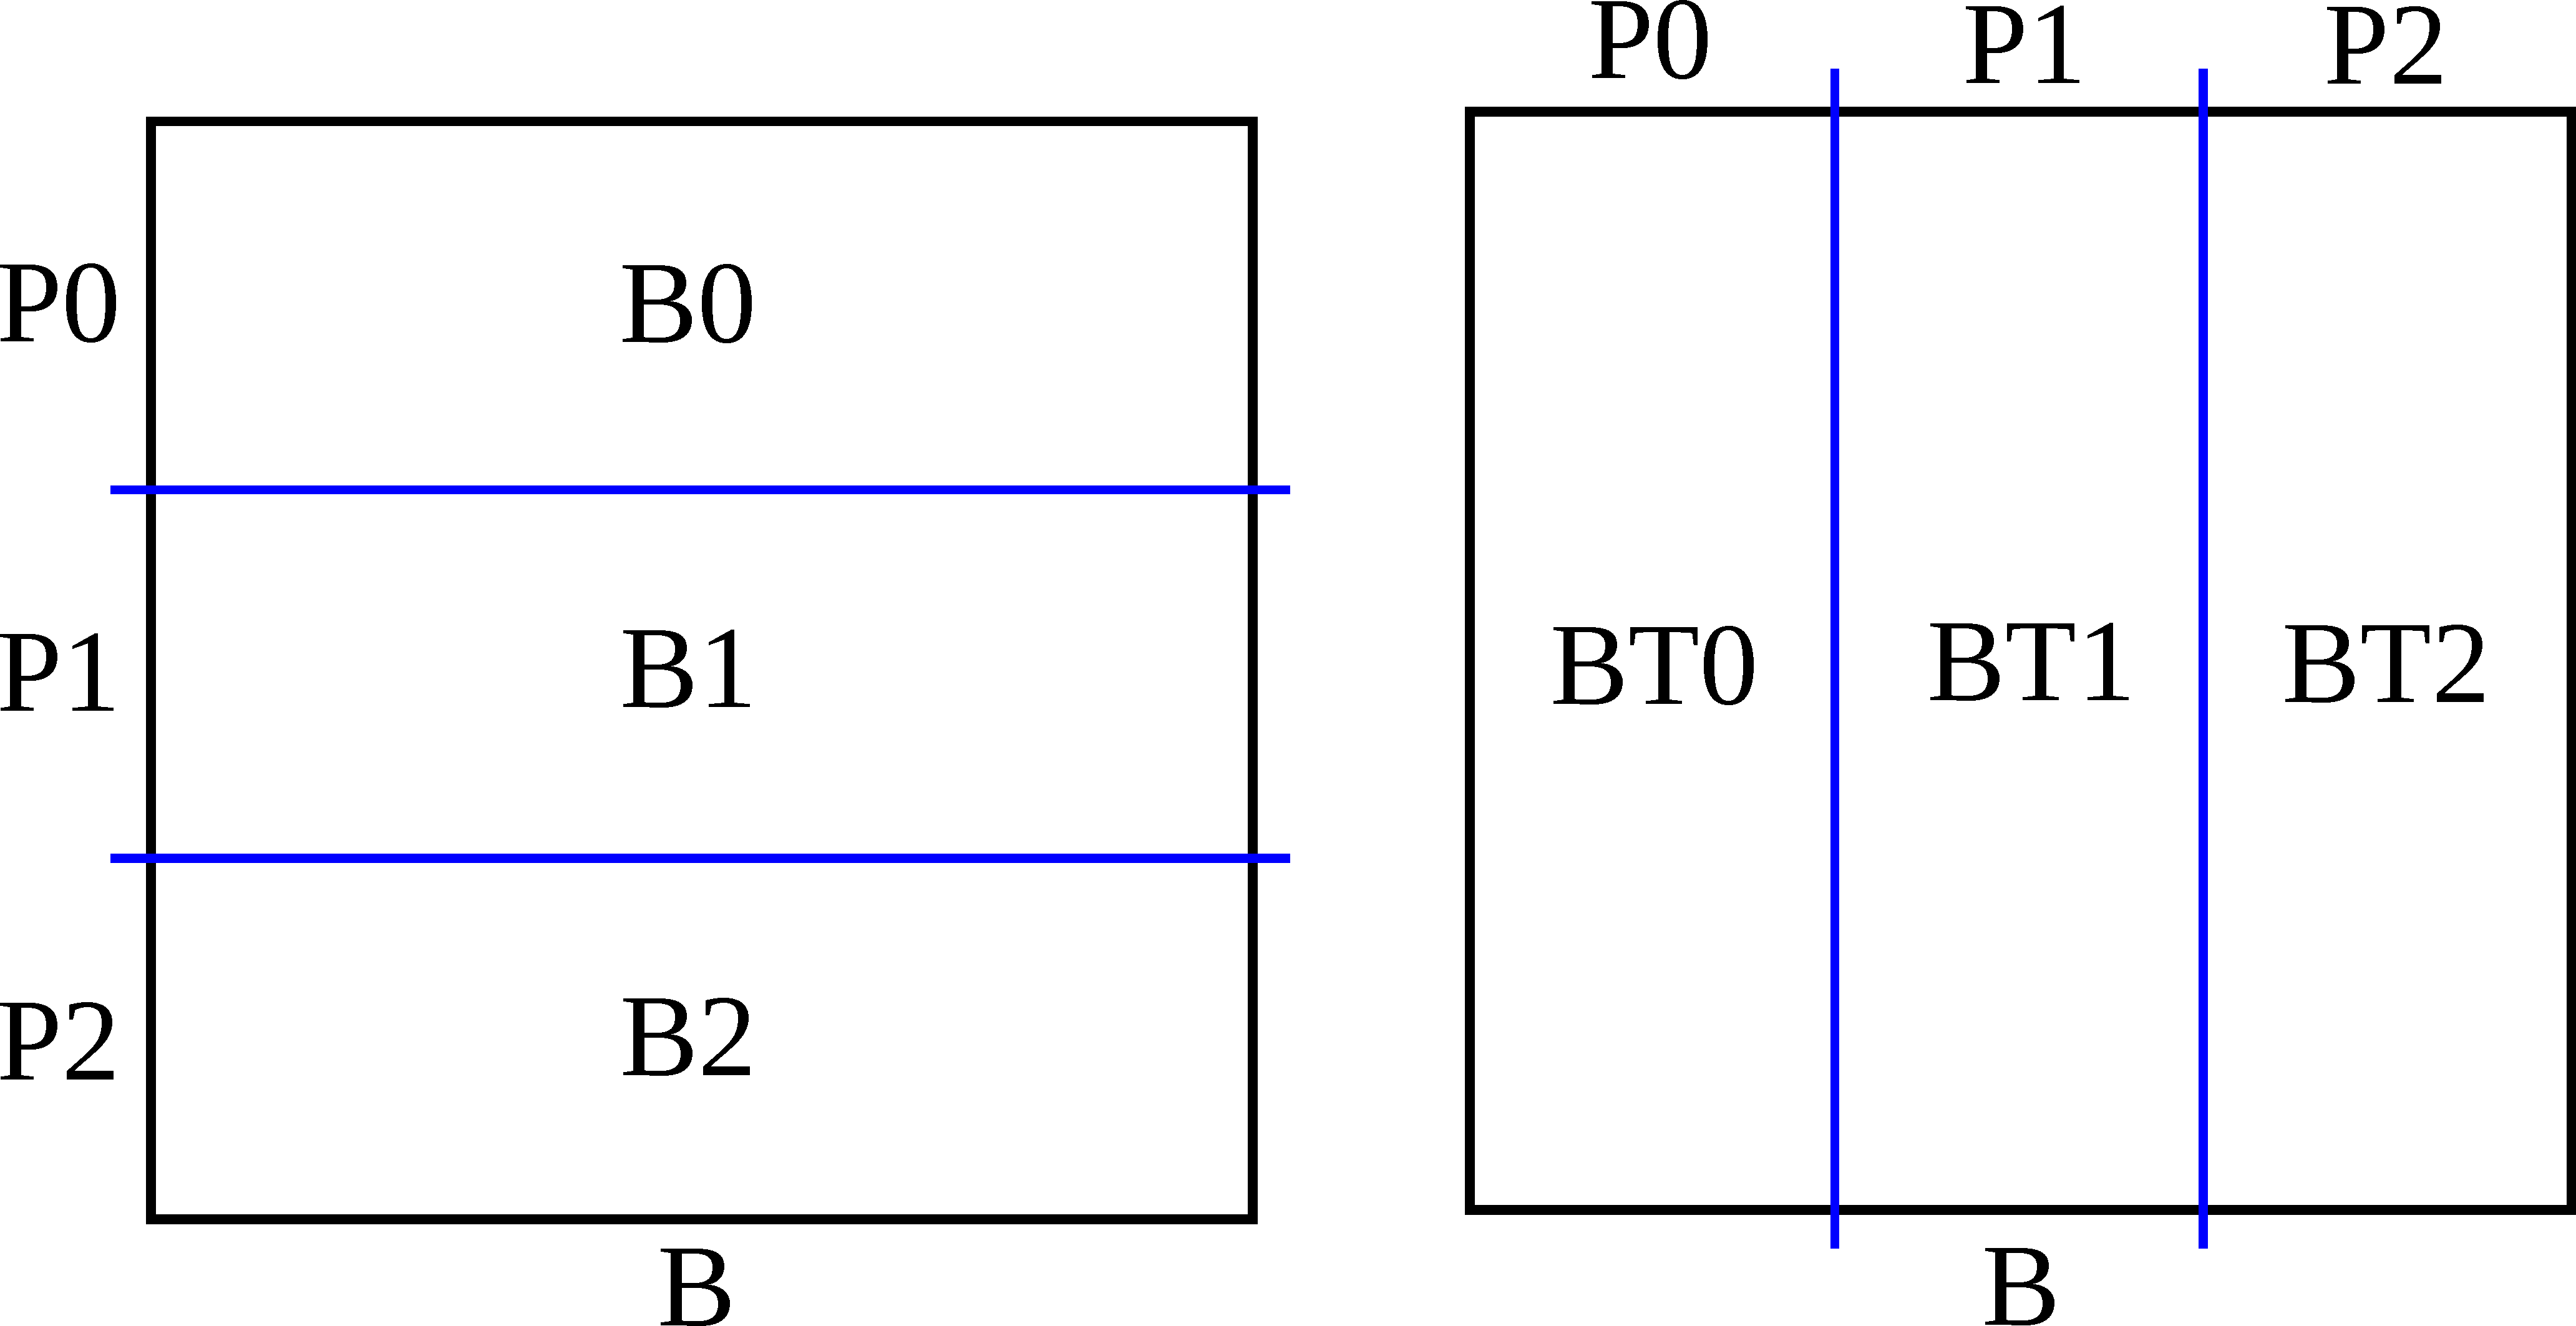
\includegraphics[width=8cm,height=4cm]{./figures/partition4.pdf}
    \caption{When $B$ is symmetric, we use local transpose of its row blocks.}
    \label{fig:partition4}
\end{figure}

If we partition $B$ in column blocks, then we don't even need $B$ to be symmetric, but since we want to consider the same partitioning method for all the matrices in our algorithm and we don't want to change the partition for one matrix to do \mm~ only, we assume $B$ is symmetric.

\begin{algorithm}[H] 
  %\footnotesize
  \caption{$C_i = A_i \times B$, when $B$ is symmetric.}
  \begin{algorithmic}[1]
    \Require $A_i$, $B$
    \Ensure  $C_i$ (result of $A_i \times B$)
    \State $B\_send \leftarrow$ local transpose of $B_i$
    \For{$k=myrank:myrank+nprocs$}
      \State $Isend(B\_send)\ to\ left\ neighbor$
      \State $B\_recv \leftarrow$ Irecv(remote $B$) from right neighbor
      \State $C_{ik} \leftarrow \recmm(A_i, B\_send)$ 
      \State $wait\ for\ Isend\ and\ Irecv\ to\ finish$
      \State $swap\_pointers(B\_send,B\_recv)$
      \State locally sort $C_{ik}$ and add duplicates
    \EndFor
    \State put all $C_{ik}$'s into $C_i$
  \end{algorithmic}
  \label{alg:comm2} 
\end{algorithm}

\begin{figure*}[!thb]
    \centering
    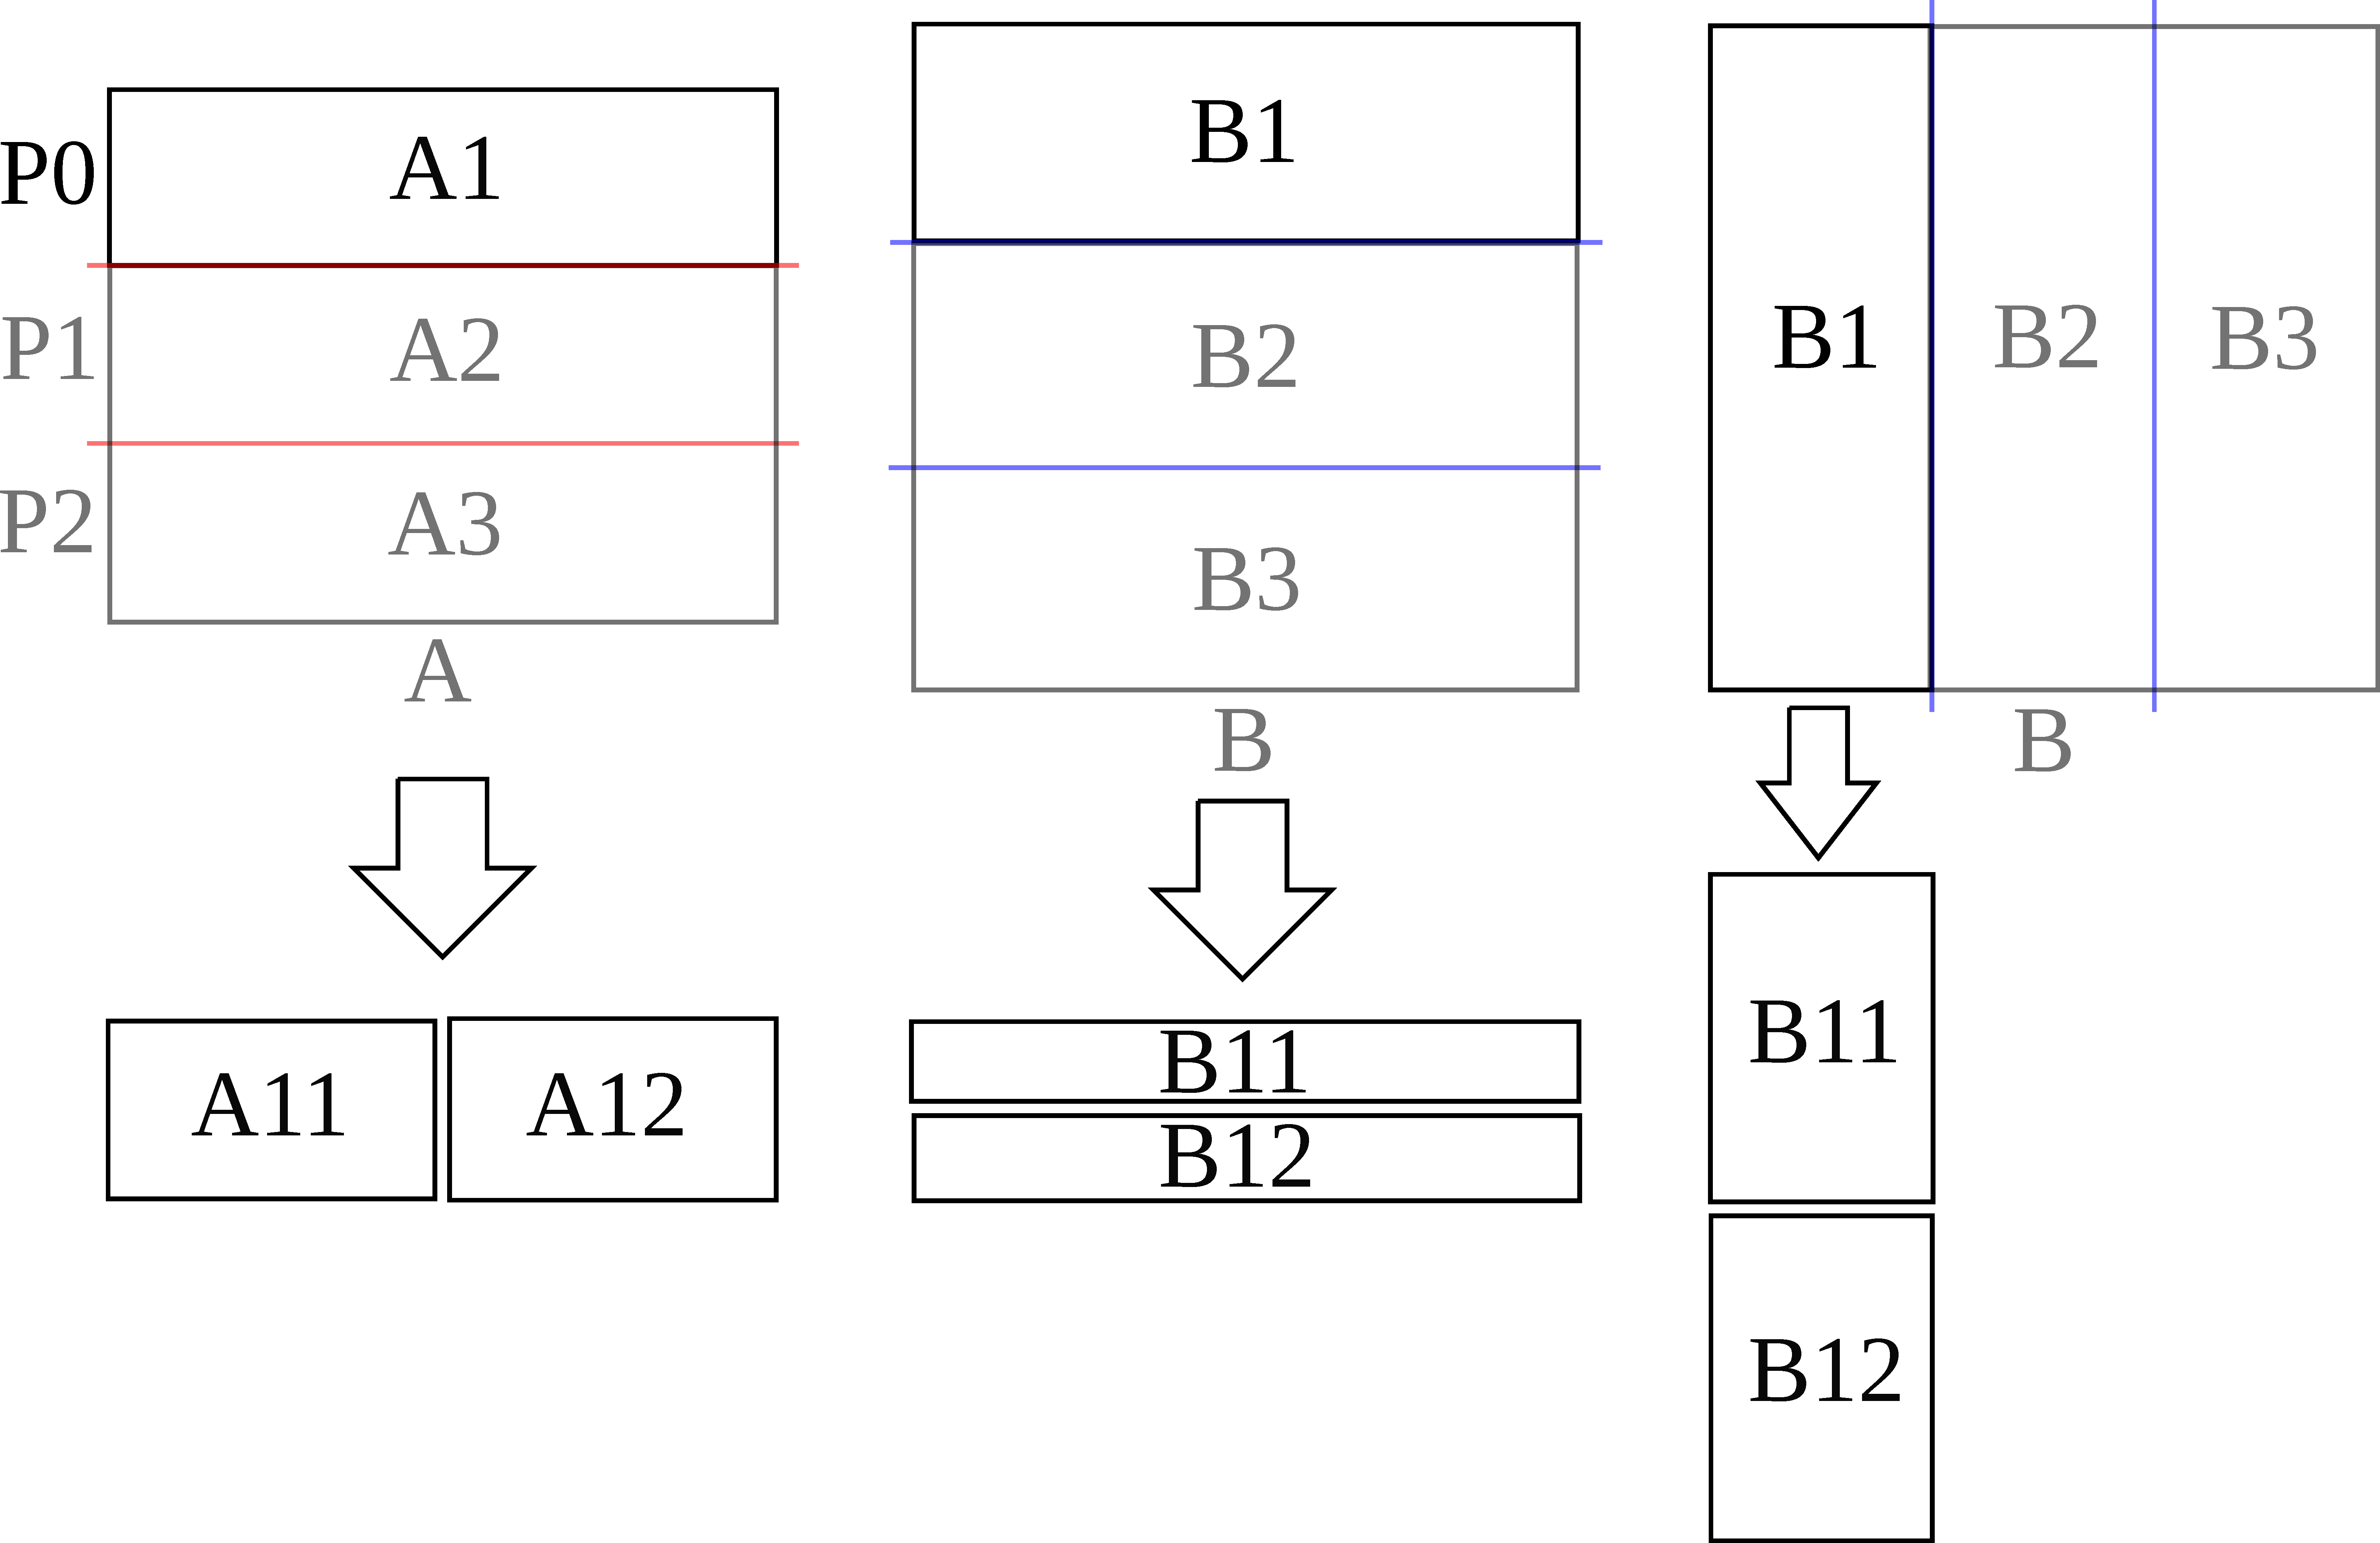
\includegraphics[width=9.4cm,height=5.8cm]{./figures/partition6.pdf}
    \caption{Comparing splitting $B$ based on Algorithm~\ref{alg:comm1} (middle) and Algorithm~\ref{alg:comm2} (right)}
    \label{fig:partition6}
\end{figure*}

There are at least two advantages for using Algorithm~\ref{alg:comm2} instead of Algorithm~\ref{alg:comm1}. First, we can sort subsets of entries of $C_i$ separately and add duplicates (compare line 9 of Algorithm~\ref{alg:comm1} with line $8$ of Algorithm~\ref{alg:comm2}, which is cheaper than doing that on the final matrix. The other advantage is having better divided blocks of $B$ for \recmm. The way the splitting procedure is being executed, it is more efficient to have matrix $B$ horizontal if $A$ is vertical and vice versa. Figure~\ref{fig:partition6} compares both ways of dividing matrix $B$ on processor $P0$. Algorithm~\ref{alg:comm1} makes $B$ skinnier, but Algorithm~\ref{alg:comm2} helps to reach the threshold faster.



\subsection{Comparison of the Splitting Methods}
\label{sec:compare}

In this section we compare \textit{Case 2} (vertical split) with \textit{Case 3} (horizontal split). Starting with the advantage of \textit{Case 2}, it consists of $2$ recursive calls, but \textit{Case 3} has $4$. So the cost of preparing for the recursive calls and also the cost of function calls themselves are half in \textit{Case 2}. 

Splitting vertically (\textit{Case 2}) has a property that makes it less scalable than \textit{Case 3}. Consider the simplest case, Figure \ref{fig:skinny1}, splitting $A$ vertically once and we assume this is done in serial. When $A1 \times B1$ and $A2 \times B2$ are computed, they should be added together to have the final result in $C$. This process, adding the duplicates, has at least three disadvantages. First, more entries are being stored, because of the duplicates of the nonzeros. Second, we need to perform the sorting on a multiple of number of nonzeros of $C$, to prepare for the duplicate addition step. And finally, adding the duplicates. Also note that in the worst case, the size of the result data before adding the duplicates would be: \textit{number of vertical splits} $\times$ \textit{nnz(C)}. \mr{add a figure to clarify this claim.} 

The other problem with \textit{Case 2} is that, the dense buffer needed to do $A1 \times B1$ is of size $m \times n$, which is the same as the total size of the result matrix $C$. The same is true for the second part of the multiplication, $A2 \times B2$. In other words, the dense buffer is of size \textit{row size of A} $\times$ \textit{column size of B}, so performing \textit{Case 2} does not help reaching the recursion threshold.
But, after each horizontal split, the sizes of submatrices get closer to the threshold in the factor of $4$, because of halving $A$ row-wise and halving $B$ column-wise.
%It means we need to split the matrices to smaller submatrices following the other splitting method to reach the threshold, and obviously the longer the recursive sequence, the worse the performance gets.

As the last comparison point, we will compare the last step of the recursive function, which is extracting the nonzeros from the dense buffer.
By performing \textit{Case 3}, we can compute each block of the result matrix $C$ (see Figure \ref{fig:skinny2}) independently after calling each recursive call. So actually dense buffers are a partition of the result matrix $C$. But, for \textit{Case 2}, for each of the two recursive calls in Figure \ref{fig:skinny1} we need to extract nonzeros from two dense buffers, each as the size of the whole matrix $C$, which makes this case more expensive.

%To avoid having the mentioned issues, we will only use the horizontal split method. By doing that, we can actually compute each block of the result matrix $C$ (see Figure \ref{fig:skinny2}) independently after calling each recursive call. To compute entry $C(i,j)$ and avoiding having any duplicates, we multiply the whole row $i$ of matrix $A$, with the whole column $j$ of matrix $B$. Also, after each horizontal split, the sizes of submatrices get closer to the threshold in the factor of $4$, because of halving $A$ row size and halving $B$ column size.

\begin{figure}[thb]
    %\centering
    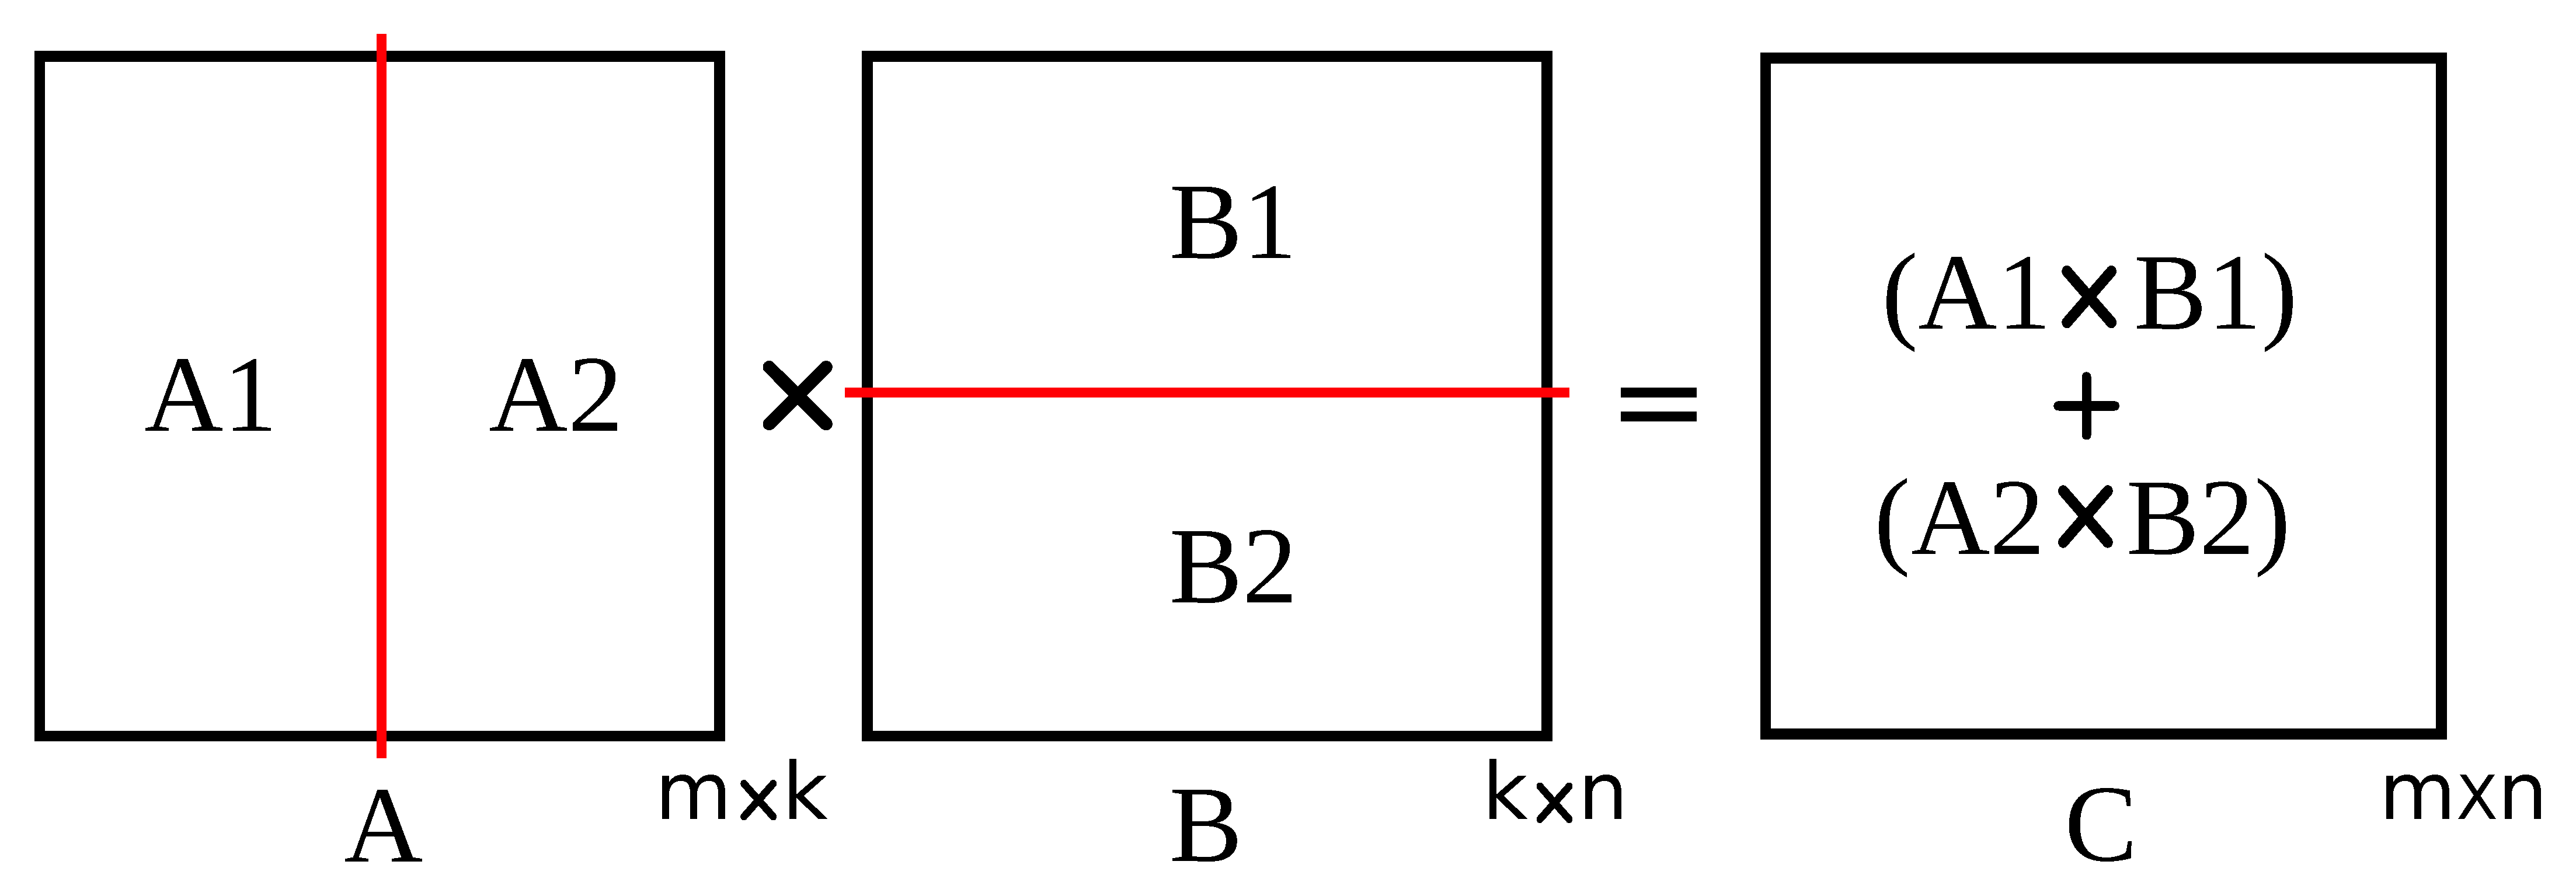
\includegraphics[width=8.8cm,height=3.1cm]{./figures/skinny001.pdf}
    \caption{Multiplication by performing \textit{Case 2} once. At the end duplicates should be added together.}
    \label{fig:skinny1}
\end{figure}

\begin{figure}[thb]
    %\centering
    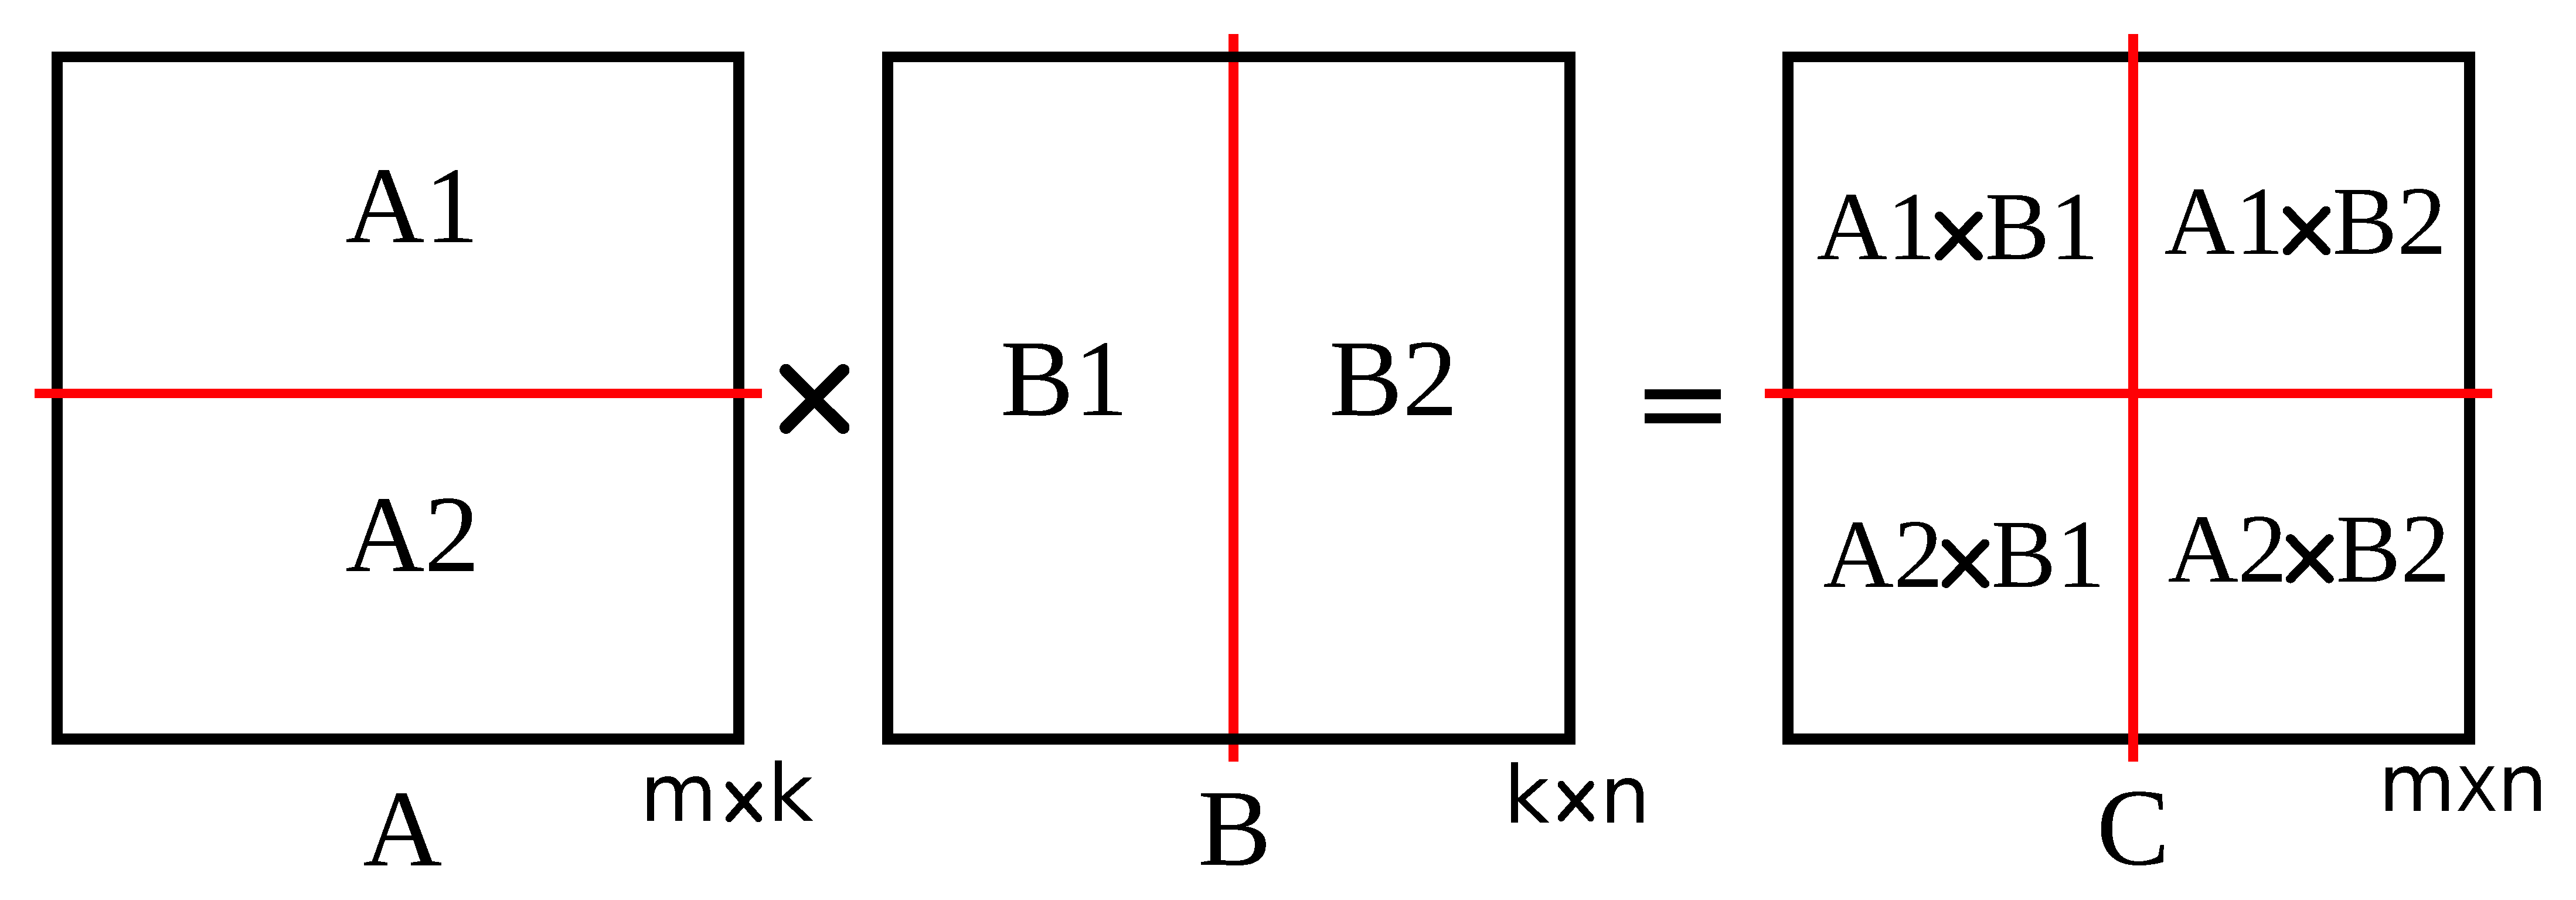
\includegraphics[width=8.8cm,height=3.1cm]{./figures/skinny002.pdf}
    \caption{Multiplication by performing \textit{Case 3} once. In this case, the dense buffers are independent and all together make a partition for the matrix $C$.}
    \label{fig:skinny2}
\end{figure}




\iffalse
\subsection{Skinny Split}
\label{sec:1split}

\mr{move some of the plots from the results section to the end of the previous section and explain where our method was not scaling well. Repeat those experiments with this new method and add these new ones to the result section.}

Splitting vertically (\textit{Case 2}) has a property that makes the method unscalable. Consider the simplest case, Figure \ref{fig:skinny1}, splitting $A$ vertically once and we assume this is done in serial. When $A1 \times B1$ and $A2 \times B2$ are computed, they should be added together to have the final result in $C$. This process, adding the duplicates, has at least three disadvantages. First, more entries are being stored, because of the duplicates of the nonzeros. Second, we need to perform the sorting on a multiple of number of nonzeros of $C$, to perform the duplicate addition step. And finally, adding the duplicates. Also note that in the worst case, the size of the result vector before adding the duplicates would be \textit{number of vertical splits} $\times$ \textit{nnz(C)}. \mr{add a figure to clarify this claim.}

The other problem with this case is that, the dense buffer needed to do $A1 \times B1$ is of size $m \times n$, which is the same as the total size of the result matrix $C$. The same is true for the second part of the multiplication, $A2 \times B2$. In other words, the dense buffer is of size \textit{row size of A} $\times$ \textit{column size of B}, so performing \textit{Case 2} does not help reaching the recursion threshold.
It means we need to split the matrices to smaller submatrices (this time based on the \textit{Case 3} method) to reach the threshold, and obviously the longer the recursive sequence, the worse the performance gets.

To avoid having the mentioned issues, we will only use the horizontal split method. By doing that, we can actually compute each block of the result matrix $C$ (see Figure \ref{fig:skinny2}) independently after calling each recursive call. To compute entry $C(i,j)$ and avoiding having any duplicates, we multiply the whole row $i$ of matrix $A$, with the whole column $j$ of matrix $B$. Also, after each horizontal split, the sizes of submatrices get closer to the threshold in the factor of $4$, because of halving $A$ row size and halving $B$ column size.

\begin{figure}[thb]
    %\centering
    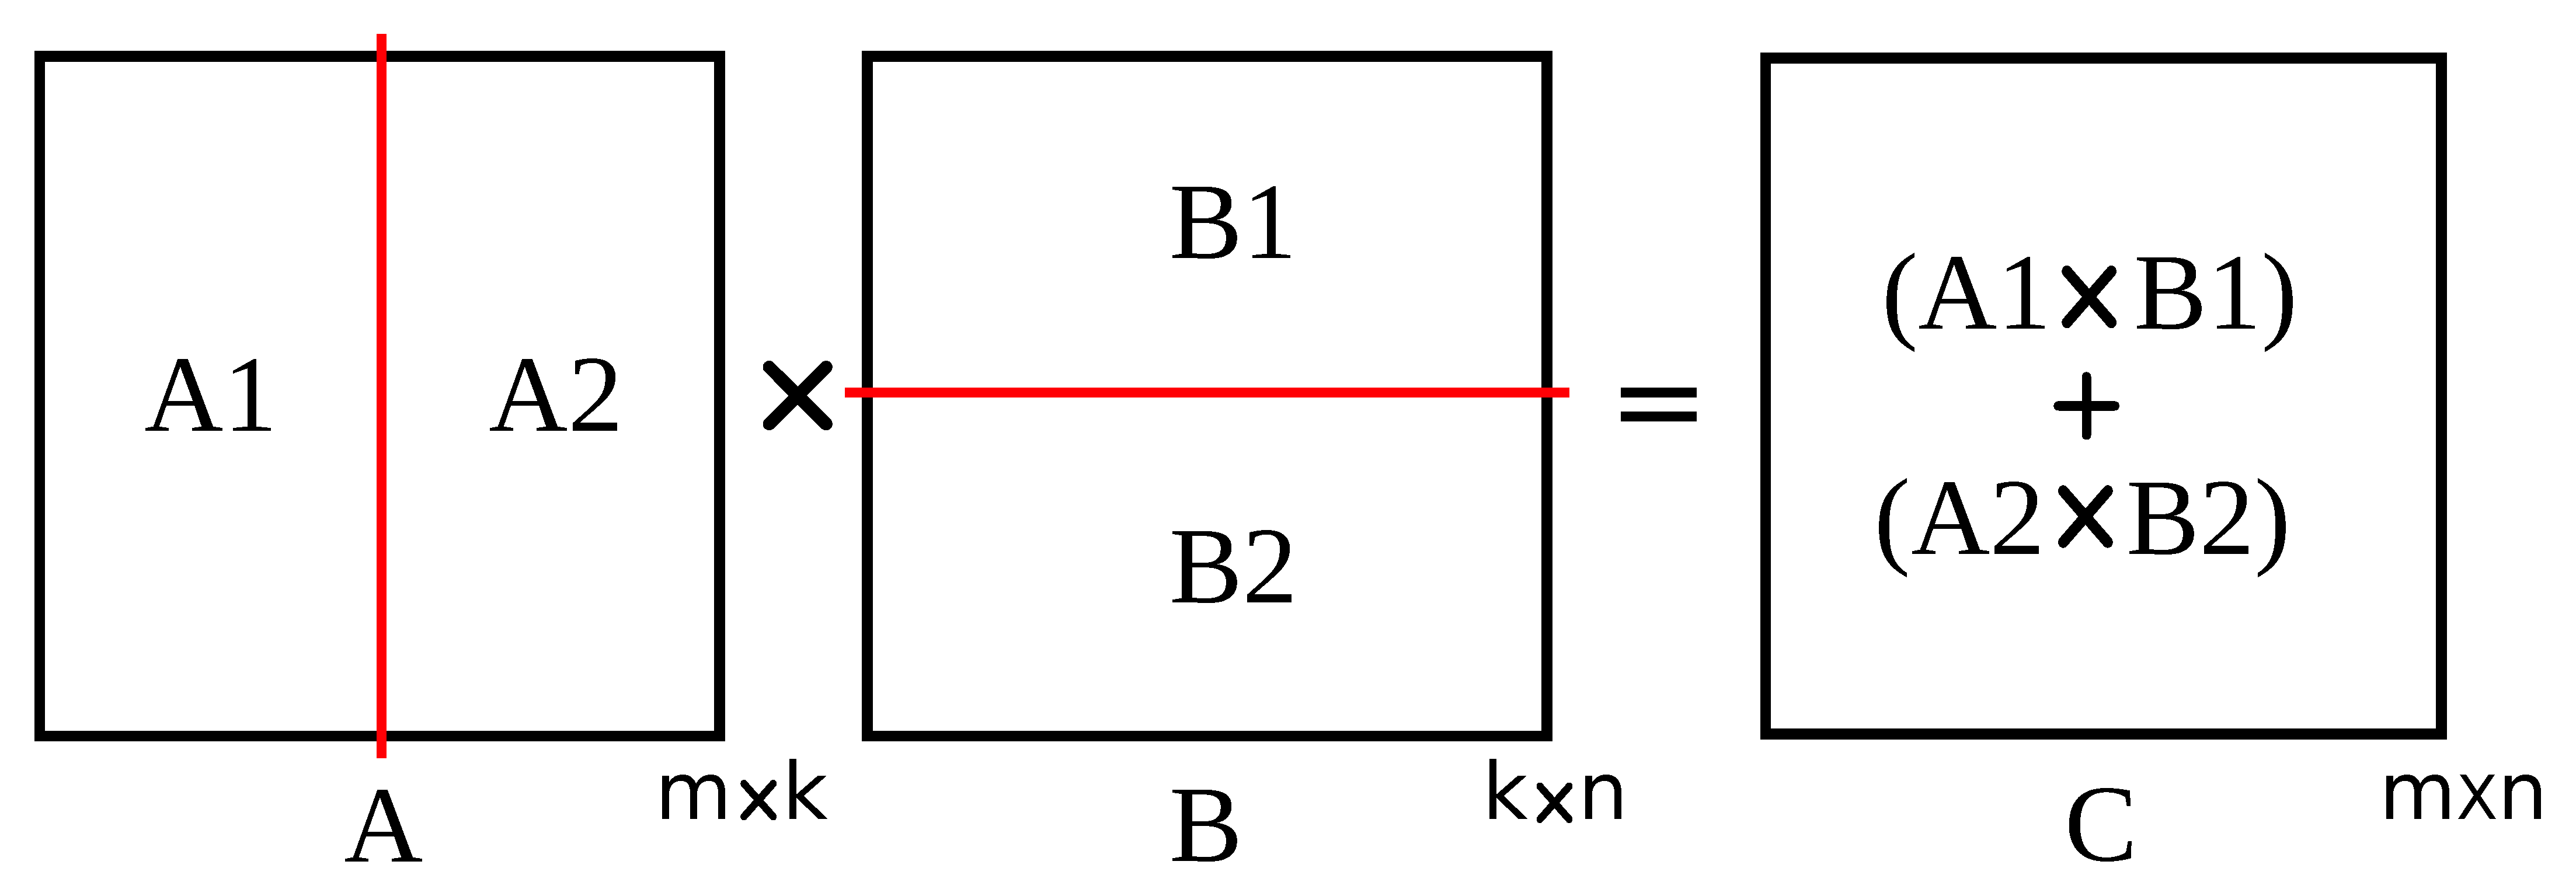
\includegraphics[width=8.8cm,height=3.1cm]{./figures/skinny001.pdf}
    \caption{Multiplication by performing \textit{Case 2} once. At the end duplicates should be added together.}
    \label{fig:skinny1}
\end{figure}

\begin{figure}[thb]
    %\centering
    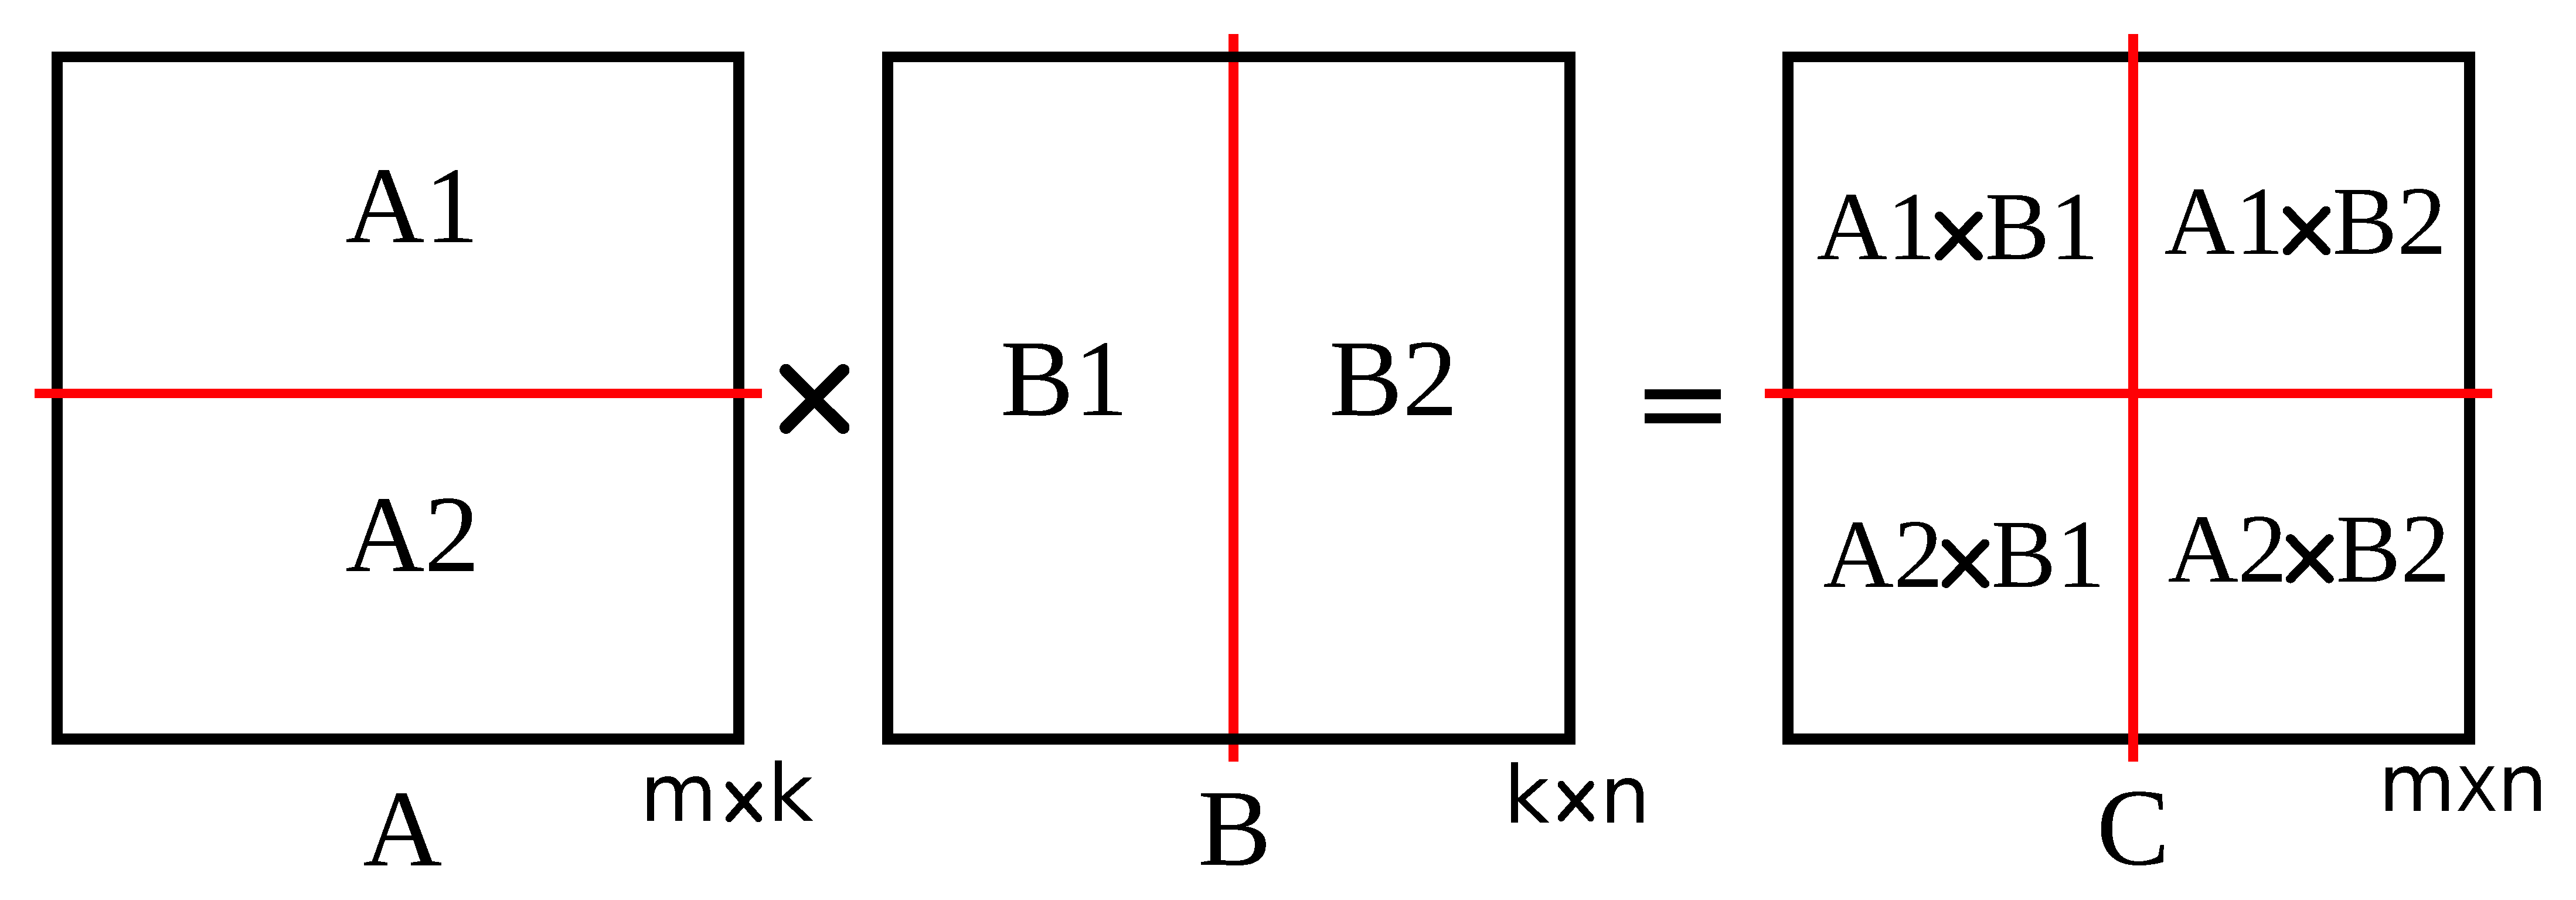
\includegraphics[width=8.8cm,height=3.1cm]{./figures/skinny002.pdf}
    \caption{}
    \label{fig:skinny2}
\end{figure}

\fi

%Talk about the steps to compute nonzero rows of A, nonzero columns of B. Then explain why using CSR for A would help.
%To further improve the scalability of our method, we change the data format for storing matrix $A$. Since in this section we want to iterate through rows of $A$ and columns of $B$, we have the matrix $A$ in the \textit{CSR} (compressed sparse row) format and matrix $B$ in \textit{CSC} (compressed sparse column) format. Recall that the matrices were in \textit{CSC} in the previous section. Following this change in storing matrix $A$, we gain another speed-up. Also recall that to stop the recursion we check:
%\begin{equation*}
%  \textit{\#nonzero rows of A} \times \textit{\#nonzero columns of B} < threshold 
%\end{equation*}

%Since $B$ was in the CSC format, we could quickly find how many columns of $B$ are nonzero. But for $A$ we had a loop of complexity $O(nnz(A))$ to compute the number of nonzero rows of $A$. Note that we could not compute it once and use it for all the next recursive call, because splitting based on \textit{Case 2} would make that invalid.

